\cleardoublepage
\chapter{Slip detection methods}\label{sec:methods}

\section{Event rate analysis}

\subsection{Introduction}

We know that if there is no slip, the object moves along with the gripper and camera, therefore, there will not be any moving edges in the event images. On the contrary, if slip occurs, moving edges will appear depending on the texture of the grasped object.\\

Thus, it might be interesting to analyze the event rate coming from the object, which may increase significantly depending on if there is slip or not. As the object may change its shape significantly from the camera's view during the slip, it is challenging to focus only on the events generated by the object. Also, events may be produced by changes in illumination, for that, it may also be informative and more robust to analyze the ratio between the events produced by the object and the total number of events.

\subsection{Results with Gelsight dataset}

To verify the aforementioned idea, first, the described event rate was analyzed with an existing dataset ~\cite{gelsight2018}, which is suitable for an initial analysis as the sequences are formed just by the initial 1 second of the lifting phase with a uniform background, including daily use objects. Nevertheless, the data contains only RGB frames coming from a standard webcam. Therefore, these sequences of images should be converted into events, which has been done using \textit{v2e} ~\cite{v2e}. This algorithm gets the events from a RGB video, first converting the frames to grayscale and then slowing down the video (by interpolating the frames) in order to compute the events with a lower latency.\\

For object 1 of the dataset and using a gripper width of 66.6 mm, the grasp is perfect and no slip occurs, as observed in ~\Cref{fig:gelsight_case1}. This case is labeled as "ok" in the dataset, meaning that the grasp occurred successfully. In addition, as the background is quite uniform, nearly no events are generated from it and only some appear from the borders of the table.

\begin{figure}[H]
    \centering
    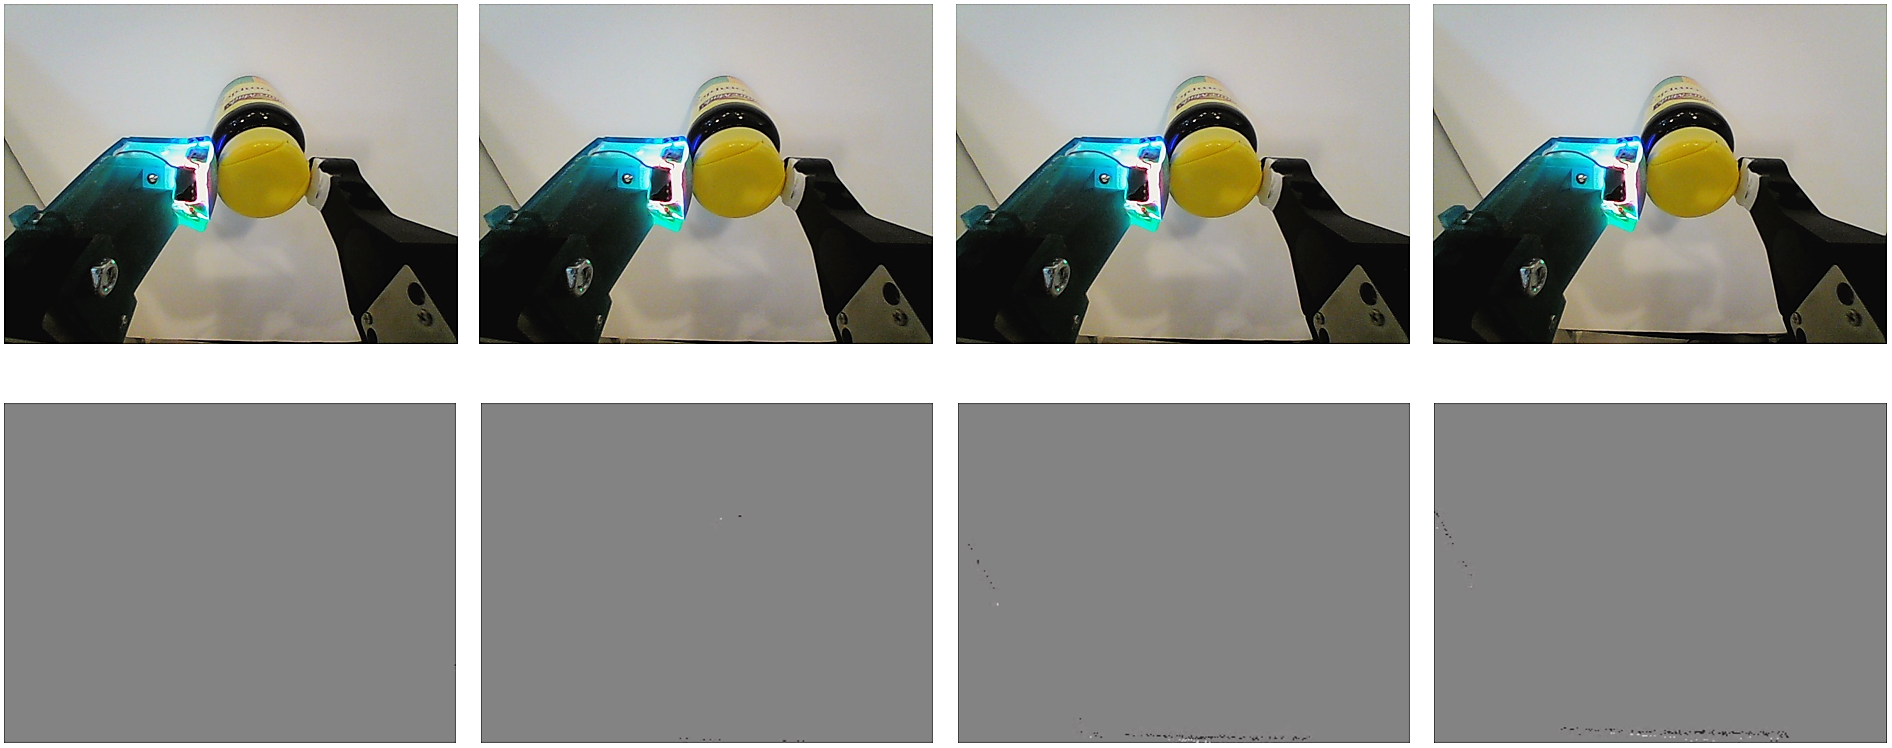
\includegraphics[width=\textwidth]{resources/images/gelsight_case1}
    \caption{Sequence of RGB frames (first row) and event images (second row) with object 1 from the dataset in ~\cite{gelsight2018} and a gripper width of 66.6 mm.}\label{fig:gelsight_case1}
\end{figure}

Opening a bit more the gripper, concretely with a width of 67.2 mm, the grasp is still labeled as "ok", but some events appear in the middle of the lift, as represented in ~\Cref{fig:gelsight_case2}. Nevertheless, this minor slip does not affect the grasp and the object is lifted successfully.

\begin{figure}[H]
    \centering
    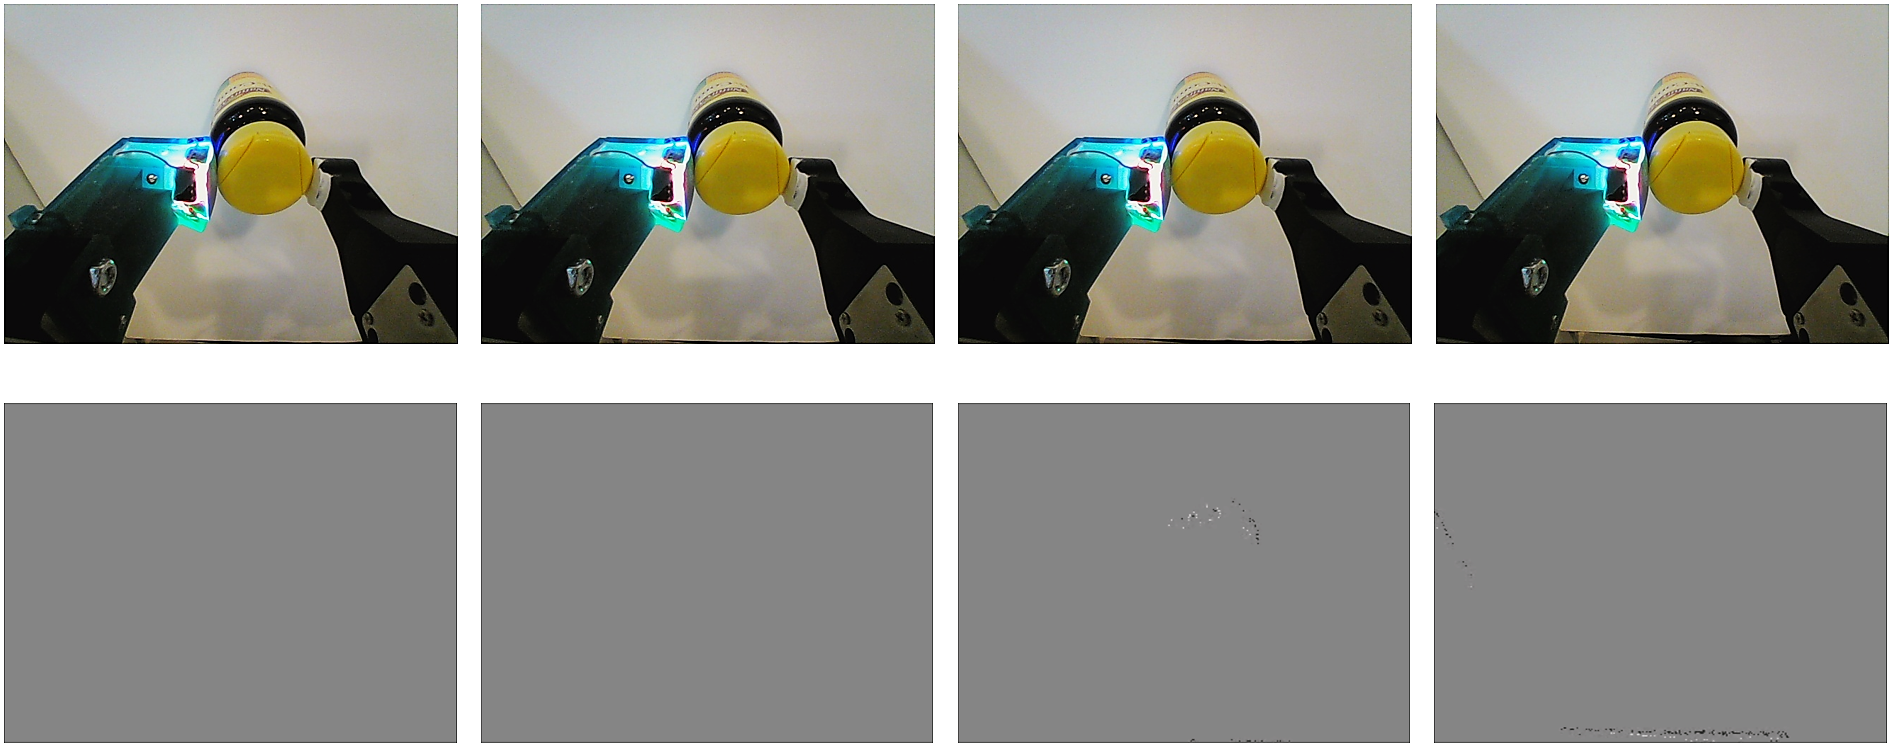
\includegraphics[width=\textwidth]{resources/images/gelsight_case2}
    \caption{Sequence of RGB frames (first row) and event images (second row) with object 1 from the dataset in ~\cite{gelsight2018} and a gripper width of 67.2 mm.}\label{fig:gelsight_case2}
\end{figure}

With a gripper width of 67.3 mm, the first sample labeled as "fail" can be found. As depicted in ~\Cref{fig:gelsight_case3}, a minor slip occurs in the beginning of the lift, then it stops slipping and just in the end the object starts falling.\\

\begin{figure}[h]
    \centering
    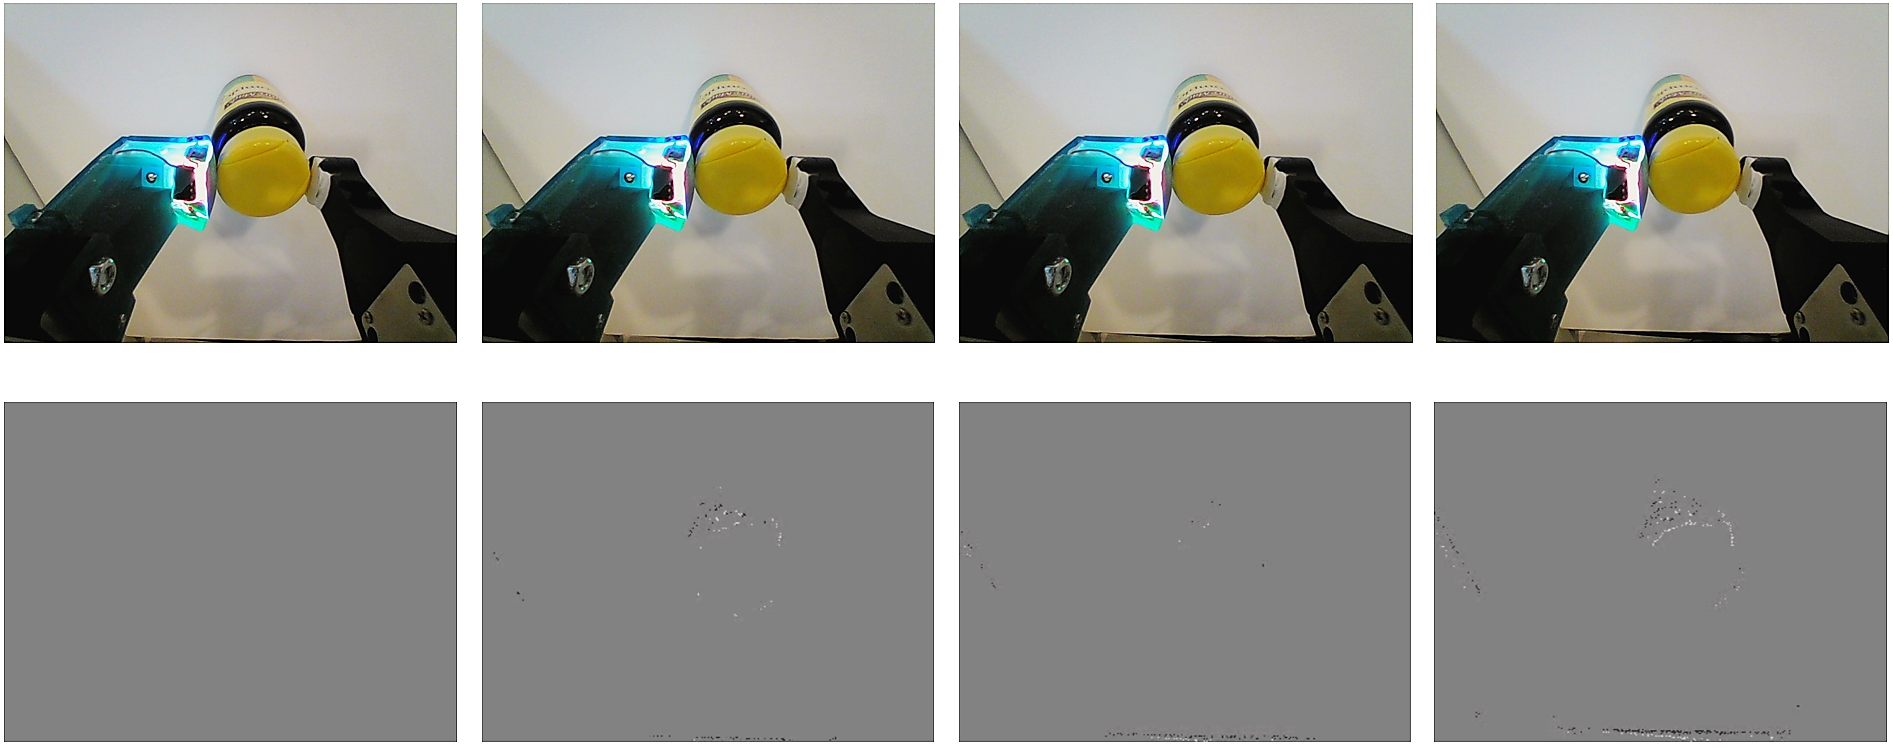
\includegraphics[width=\textwidth]{resources/images/gelsight_case3}
    \caption{Sequence of RGB frames (first row) and event images (second row) with object 1 from the dataset in ~\cite{gelsight2018} and a gripper width of 67.3 mm.}\label{fig:gelsight_case3}
\end{figure}

Finally, opening the gripper until 67.5 mm, produces a clear grasping failure, not even lifting the object, as shown in ~\Cref{fig:gelsight_case4}, where events are coming from the object continuously, while the gripper moves away from it without grasping it.\\

\begin{figure}[h]
    \centering
    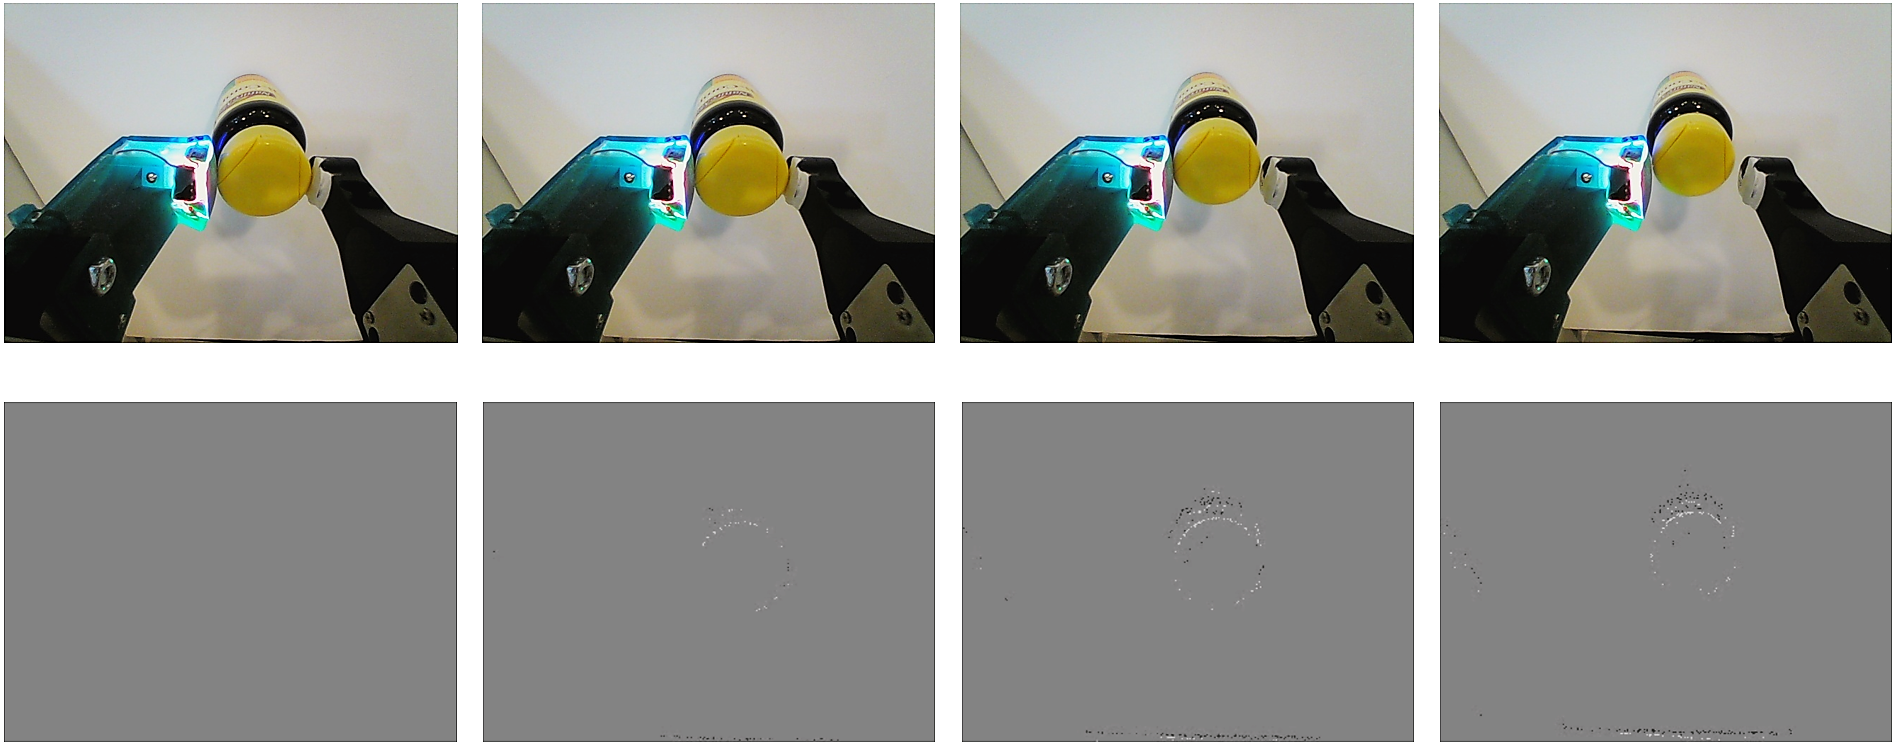
\includegraphics[width=\textwidth]{resources/images/gelsight_case4}
    \caption{Sequence of RGB frames (first row) and event images (second row) with object 1 from the dataset in ~\cite{gelsight2018} and a gripper width of 67.5 mm.}\label{fig:gelsight_case4}
\end{figure}

With these 4 samples, the event rate in the whole image can be computed as a first analysis, instead of focusing only in the object, as the background is quite uniform, thus not many events will be generated by it. Also, the background is constant in all the samples, so the events generated from it will also be the same for each sample, being the only difference the events associated to the object movement.

In ~\Cref{fig:gelsight_evr}, the evolution of the event rate in the whole image for the 4 detailed examples is shown. This event rate has been computed counting the events during consecutive time windows of 10 ms, value selected in order to have the lowest latency possible without having a really noisy signal. For the two cases labeled as "ok", similar evolutions can be observed, increasing the event rate towards the end, due to the background events. With a gripper width of 67.3 mm, there is a slip in the beginning of the lift and the event rate is higher than the previous two examples between 0.5 and 0.6 seconds due to it. Additionally, towards the end, the object starts falling and many events appear in the scene, which is reflected by the high peak in the end of the sequence. Finally, for the last experiment, the event rate is clearly higher than the other samples during the whole sequence due to the grasp failure.\\

\begin{figure}[h]
    \centering
    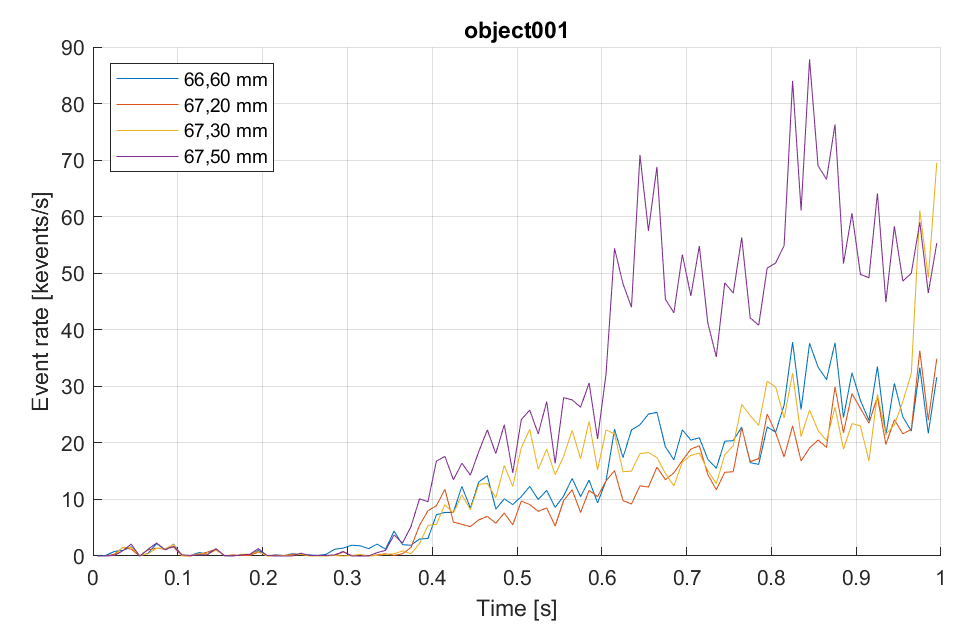
\includegraphics[width=\textwidth]{resources/images/gelsight_evr}
    \caption{Comparison of the event rate evolution in the whole image for 4 samples of object 1 from the dataset in ~\cite{gelsight2018}.}\label{fig:gelsight_evr}
\end{figure}

Thanks to this analysis, the usefulness of the event rate for slip detection is proved. For instance, if this one dimensional signal surpasses a certain threshold (40 kevents/s in this example), a slip can be detected. However, it is true that in this case the background is uniform and constant during all the experiments, this is why only with the event rate in the whole image is enough to detect slip, which may not be the case in our sets of data.\\

As an example, only the first object of the dataset has been analyzed in detail here, but the drawn conclusions apply also to other objects and experiments.

\subsection{Results with Set 1 and fixed RoI}

In our dataset, the background is not uniform, therefore, in order to detect slip we need to focus on the events coming from the object. One naive approach is to manually annotate with a rectangle where the object is in the first frame (just when the gripper has closed in the picking phase), which is denoted as the Region of Interest (RoI), and keep it fixed during the whole sequence, assuming that the object will stay in that region during the whole motion. Of course, using a rectangle is the simplest option, but it may not fit properly the object, including some parts of the background in the RoI. Also, keeping it fixed means that during the sequence, if there is a slip, the object may fall out of the RoI or more background parts fall into it. In ~\Cref{fig:fix_roi} some examples of manually annotated RoIs are depicted.

\begin{figure}[h]
    \centering
    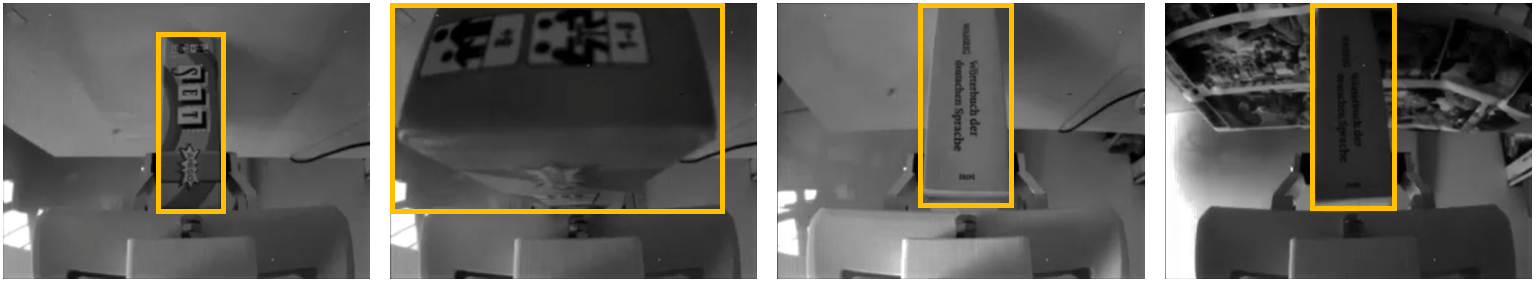
\includegraphics[width=\textwidth]{resources/images/fix_roi}
    \caption{Example initial frames of Set 1, with their respective fix RoI.}\label{fig:fix_roi}
\end{figure}

In ~\Cref{fig:fix_roi_set}, the evolution of the event rates for the RoI and the whole image have been represented, considering a time window of 10 ms, for the sequences like the ones shown in ~\Cref{fig:set1_case1} and ~\Cref{fig:set1_case2}. In addition, the ratio between these two signals is included, which is better suited to be thresholded, as it is bounded between 0 and 1. This signal can be interpreted as the relative amount of events inside the RoI compared to the whole image, which intuitively seems informative of slip cases. 

\begin{figure}[h]
    \centering
    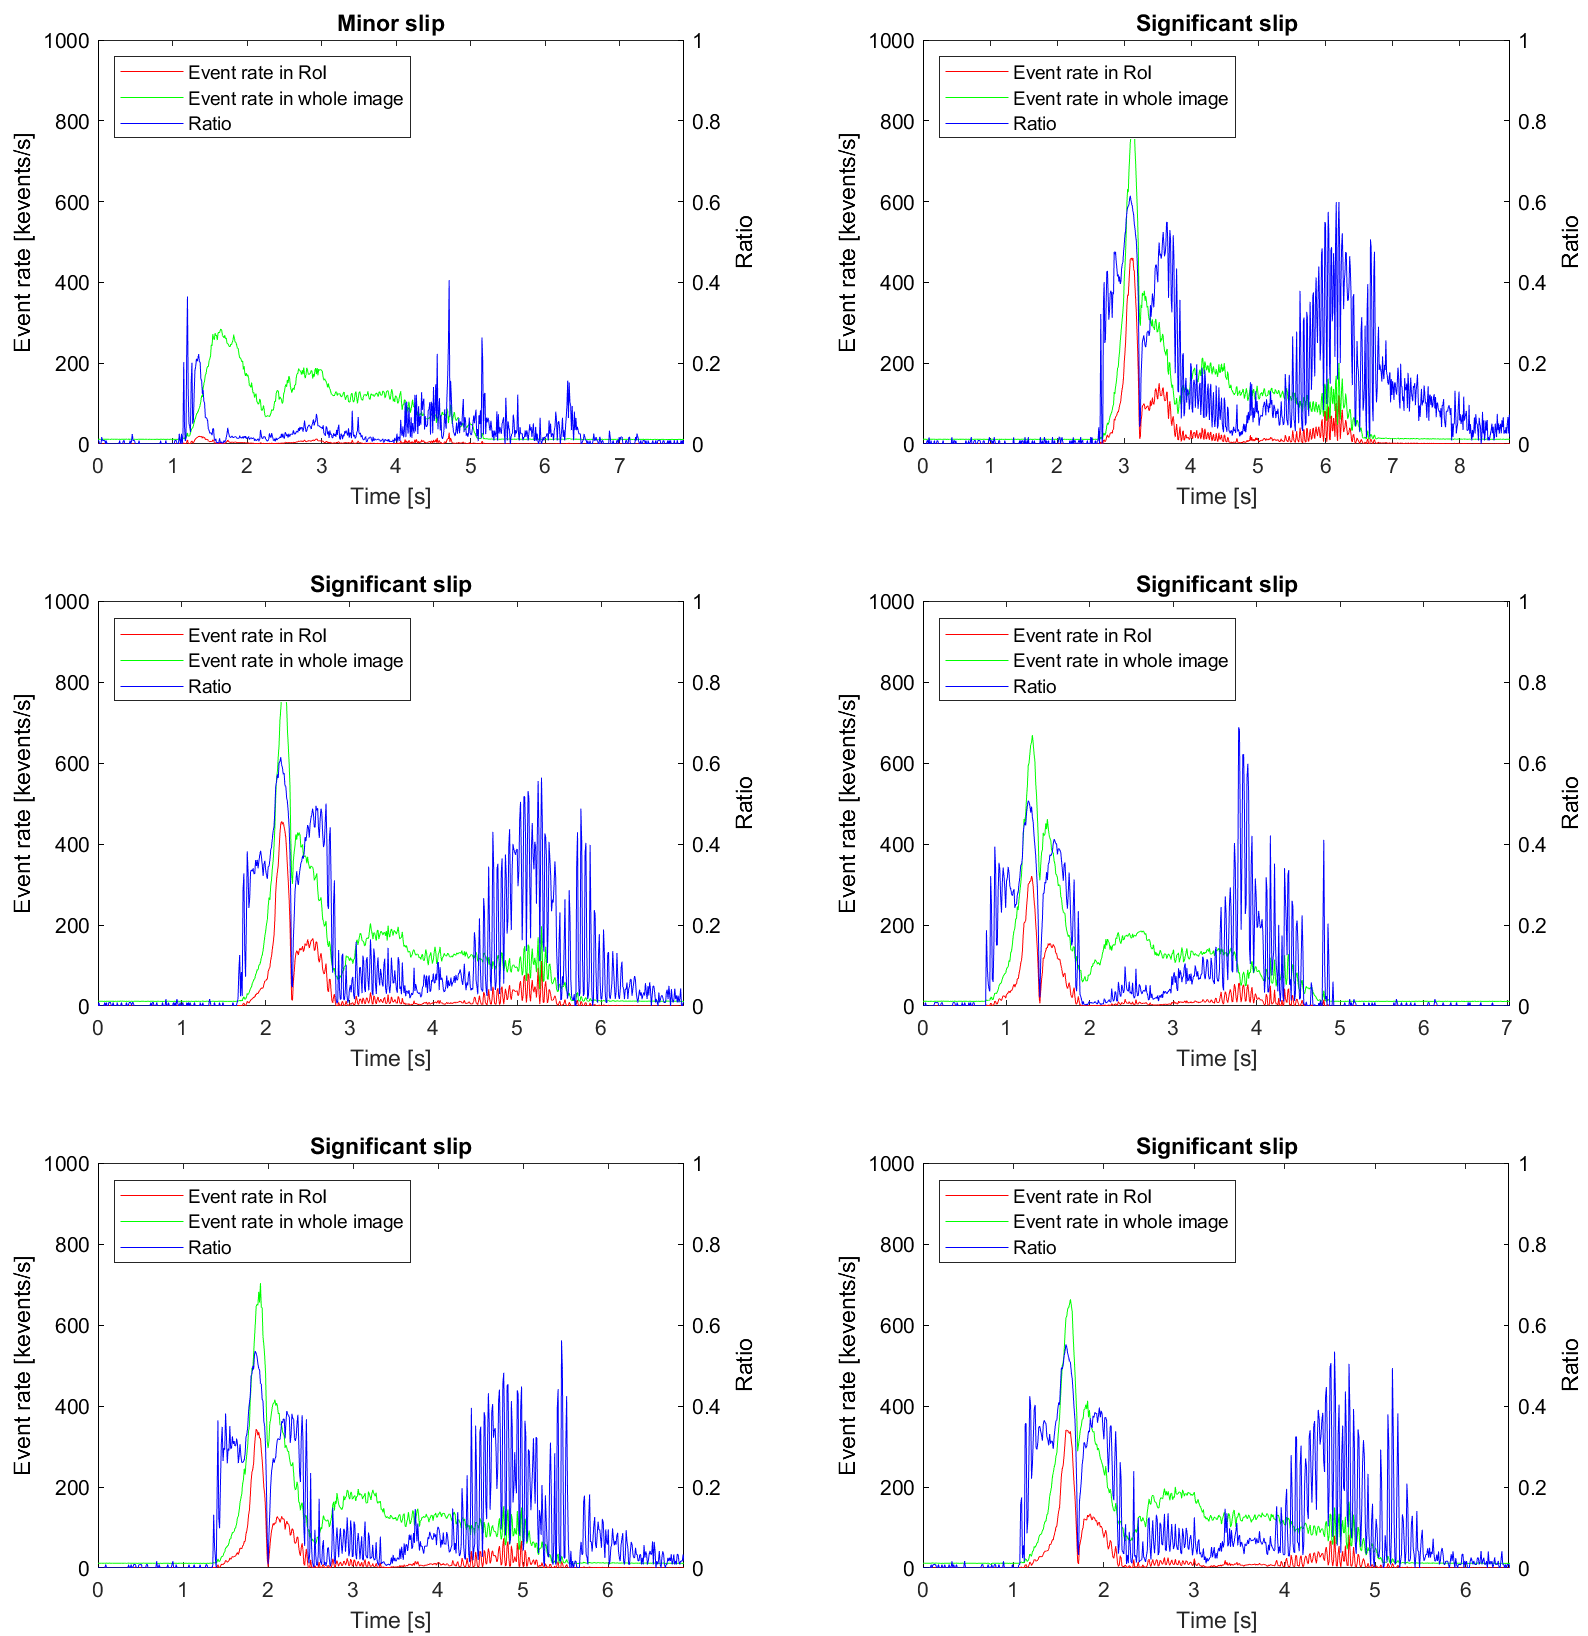
\includegraphics[width=\textwidth]{resources/images/fix_roi_set}
    \caption{Event rate and ratio signals during a pick-and-place motion with a box using a fixed RoI.}\label{fig:fix_roi_set}
\end{figure}

In terms of the minor slip case, the sequence of which was depicted in ~\Cref{fig:set1_case1}, the event rate in the RoI is really small and we can only see a small peak around 1.5 s, corresponding to the mentioned minor slip, and then another one around 4.7 s, another minor slip present in the sequence. These two increases in the event rate are also reflected in the ratio signal, reaching punctual values of nearly 0.4.\\

In contrast, all the other experiments present significant slip, as the one detailed in ~\Cref{fig:set1_case2}. There is a first peak in the event rate inside the RoI, corresponding to the first rotational slip, and then there is a slip in the opposite direction, which is reflected with a second peak in the signal. In order to change the direction of rotation, the object should stop in the middle, thus there should be no events coming from the object in that period, which is also visible between the two mentioned peaks. Moreover, towards the end of the motion there is another slip just before placing the object on the table, which is reflected also with high values in the event rate inside the RoI. It is worth noticing that all these peaks have different values, whereas the respective peaks in the ratio signal are comparable.\\

In this particular example, the ratio signal can be easily thresholded to 0.4 in order to detect significant slips. Nevertheless, the signal is quite noisy, which may provoke fluctuations in the slip detection. This issue can be solved by using a hysteresis or a low pass filter, which would attenuate also the spikes in the minor slip case.\\

Grasping the same box from the other end, we can see how the RoI occupies almost the whole image (see ~\Cref{fig:fix_roi}). As shown in ~\Cref{fig:set1_case6}, the box, after rotating, occupies a narrow part in the middle of the object, therefore, the initially fixed RoI clearly fails to separate the object from the background. This issue affects the results, reported in ~\Cref{fig:fix_roi_set_rev}, as the event rate inside the RoI and the whole image look pretty similar, resulting in a ratio signal which is high during most of the sequence, while there is only one major slip coinciding with the peak in the event rates.

\begin{figure}[h]
    \centering
    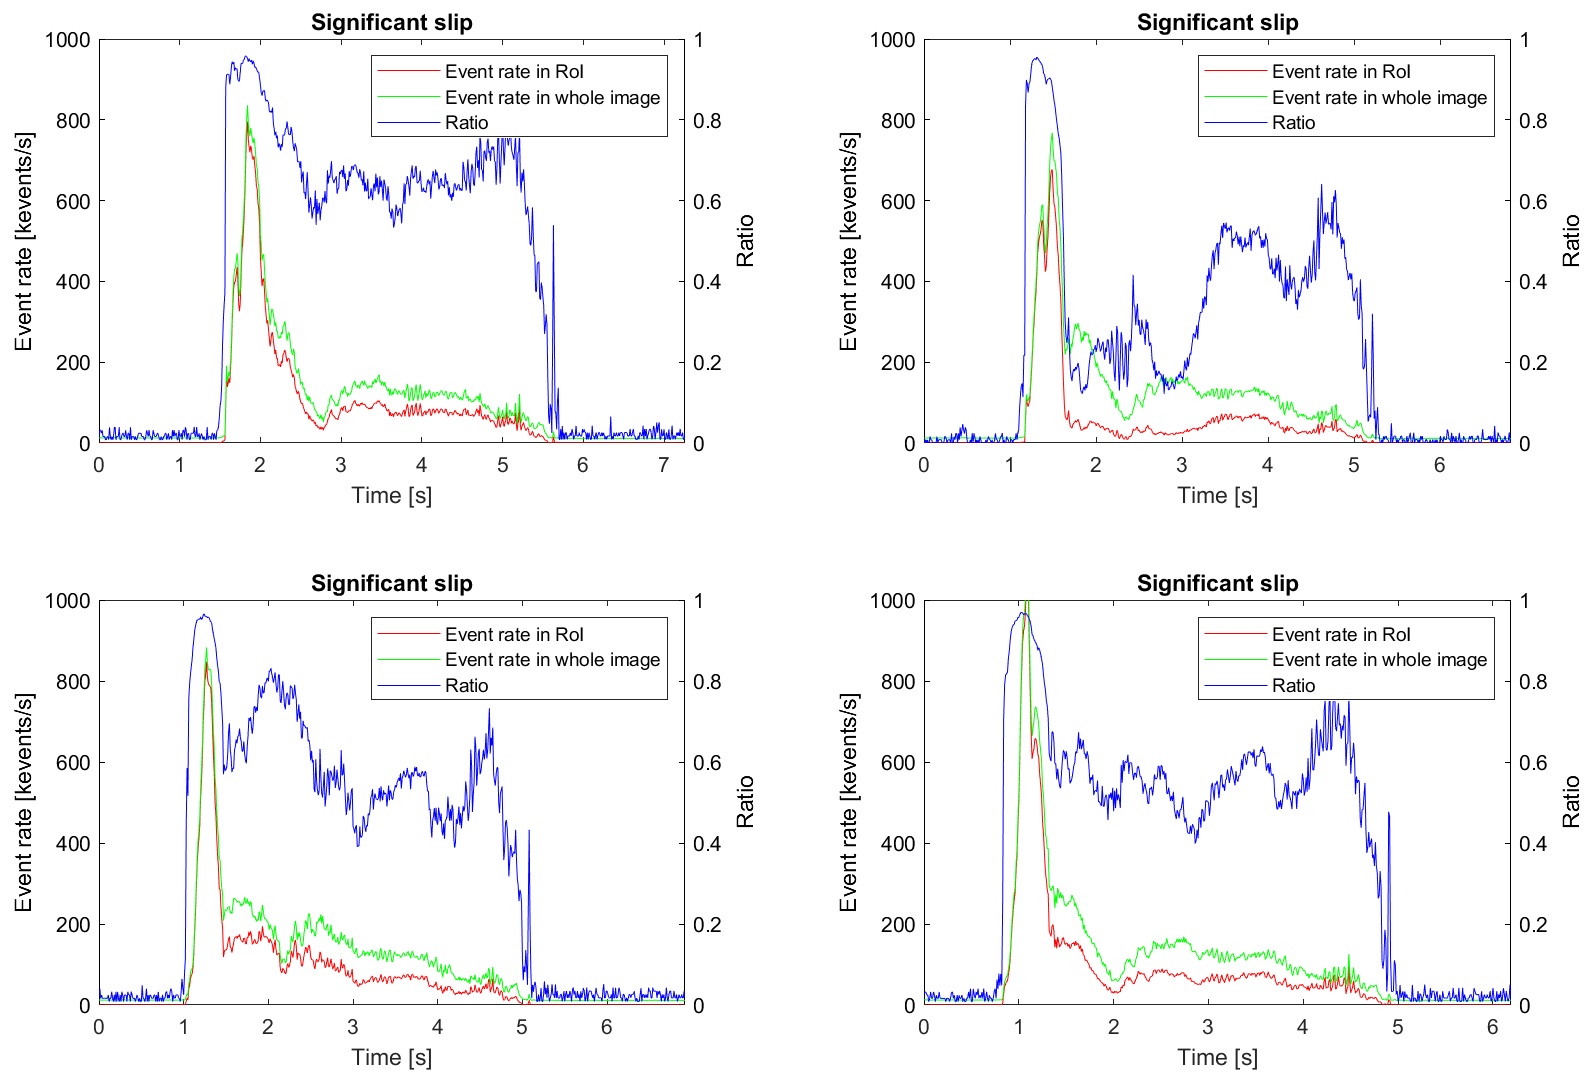
\includegraphics[width=\textwidth]{resources/images/fix_roi_set_rev}
    \caption{Event rate and ratio signals during a pick-and-place motion with a box (reverse grip) using a fixed RoI.}\label{fig:fix_roi_set_rev}
\end{figure}

Using another object, the effect of different texture can be analyzed. For instance, with sequences like the one shown in ~\Cref{fig:set1_case3}, the results reported in ~\Cref{fig:fix_roi_book1} are obtained. As detailed previously, in this sequence there is an initial slip in one direction and then in the opposite direction, which can be detected with the first two peaks of the ratio signal. Moreover, towards the end of the sequence there is a slight movement of the book, which is also detectable in the increasing ratio signal. Finally, the book is placed on the table, but due to its rotation it impacts against it, provoking the last spike in the signal. It is worth noticing how in this case, where the object has much less texture compared to the previous box, meaning that less events are generated by its movement, the ratio threshold suitable for slip detection would be around 0.2, half compared to the previous threshold.

\begin{figure}[h]
    \centering
    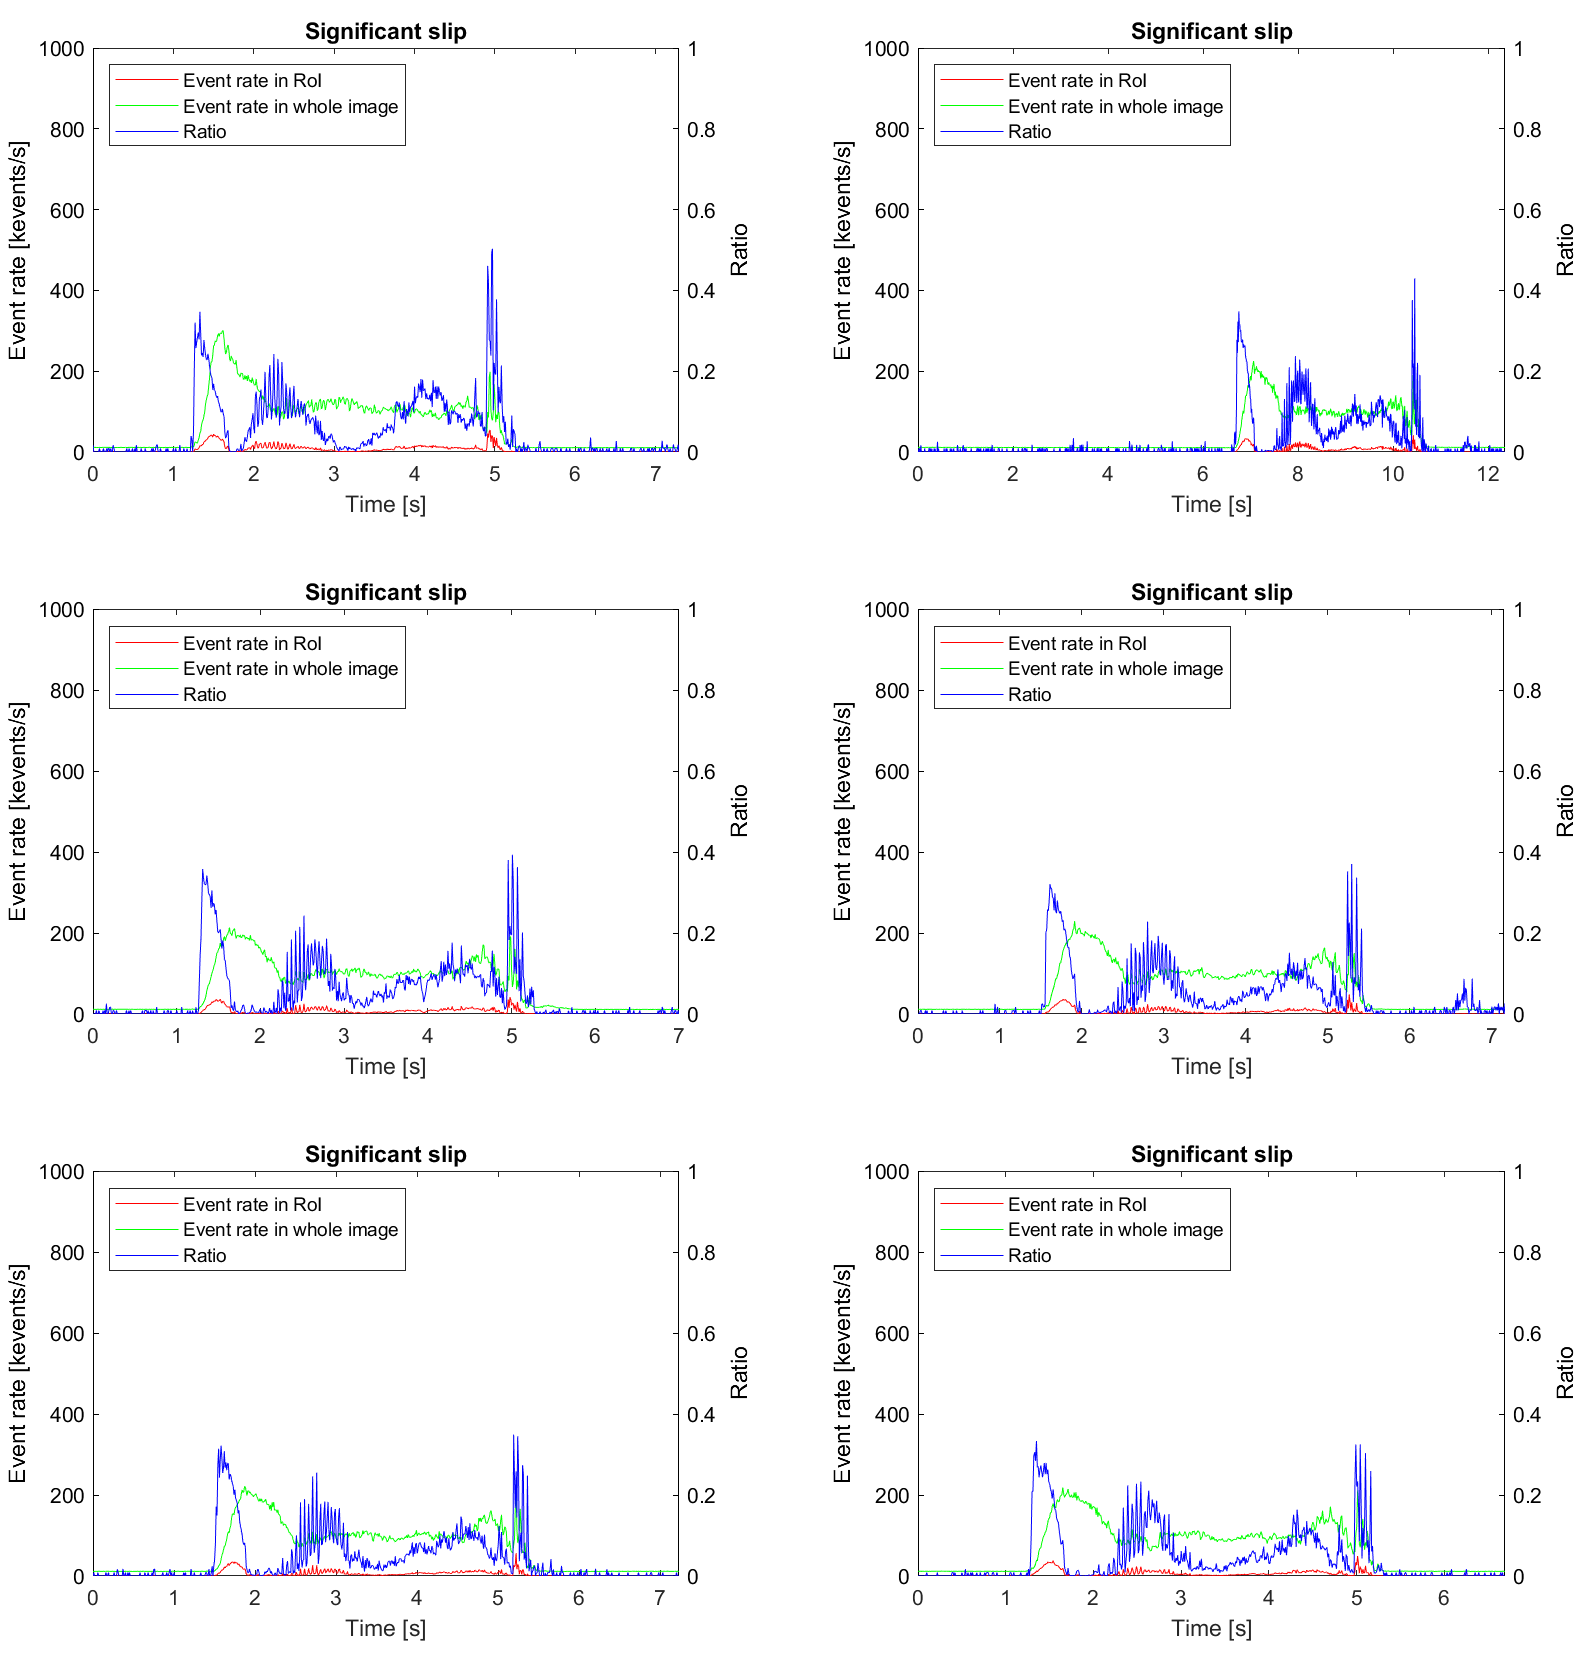
\includegraphics[width=\textwidth]{resources/images/fix_roi_book1}
    \caption{Event rate and ratio signals during a pick-and-place motion with book no. 1 using a fixed RoI.}\label{fig:fix_roi_book1}
\end{figure}

To make it more challenging, the texture of the background can be modified, as happened in the sequence depicted in ~\Cref{fig:set1_case7}, which is the same as ~\Cref{fig:set1_case3}, but adding much more texture to the table. The resulting event rate and ratio signals are reported in ~\Cref{fig:fix_roi_book1_tt}, where similar patterns in the ratio signal are observed, compared to the previous scenario, but now they are not thresholdable for slip detection, due to the high amount of events coming from the background.\\

\begin{figure}[h]
    \centering
    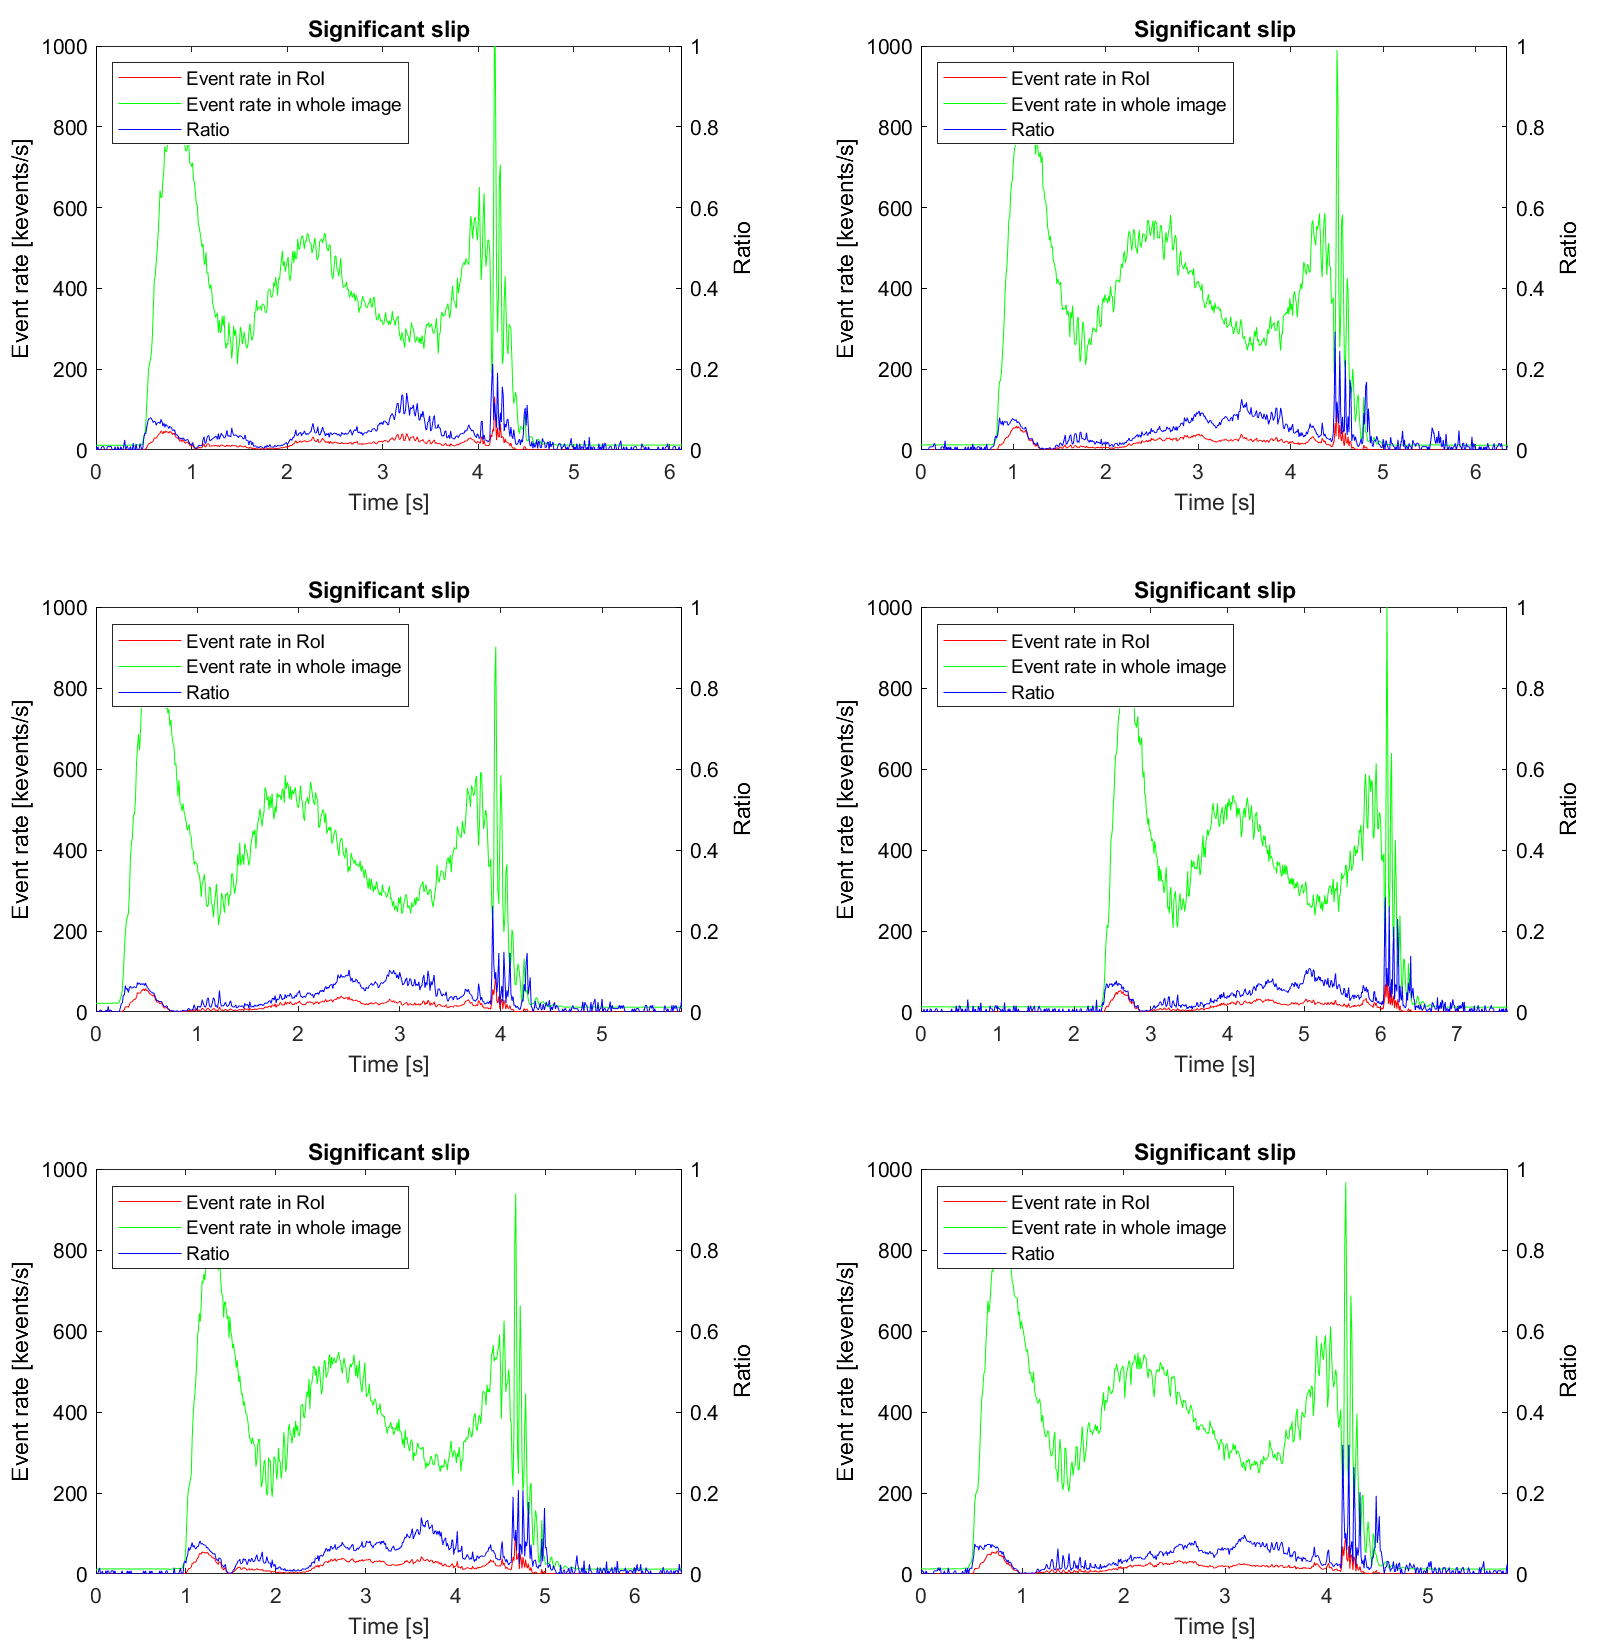
\includegraphics[width=\textwidth]{resources/images/fix_roi_book1_tt}
    \caption{Event rate and ratio signals during a pick-and-place motion with book no. 1 and a highly textured table using a fixed RoI.}\label{fig:fix_roi_book1_tt}
\end{figure}

All in all, this method presents several disadvantages, but shows the potential and limitations of using the ratio signal for slip detection. First, the ratio threshold depends on the texture of the object and also on the background. Additionally, the fixed RoI may not separate the object from the background during the whole sequence, which disables the possibility of slip detection by thresholding the ratio signal.

\subsection{Results with Set 1 and weighted mask}

Using an initially defined fixed RoI, presents the inconvenience of setting it for each scenario and not being valid for cases where the initial and final positions of the object are really different, as for the sequence ~\Cref{fig:set1_case6}. However, as the gripper position in the image plane is known, we have the prior information of where the object is going to be, i.e. between the fingers of the gripper. For each object the width of the gripper is different, but the maximum width is known, which is set as two times the standard deviation, as represented in ~\Cref{fig:gaus_mask}. Then, a Gaussian is defined with it along the horizontal direction, with a peak value of 1 in the center of the image and lower values when further from the center. These values are taken into account as weights for the events generated, which depending on the position in which they appear in the image they might have more or less importance. Moreover, the bottom part, which is mostly occupied by the gripper and the camera mount, has a null weight. With this weighted mask, a weighted histogram is computed along time, to generate the event rate and ratio signals.

\begin{figure}[h]
    \centering
    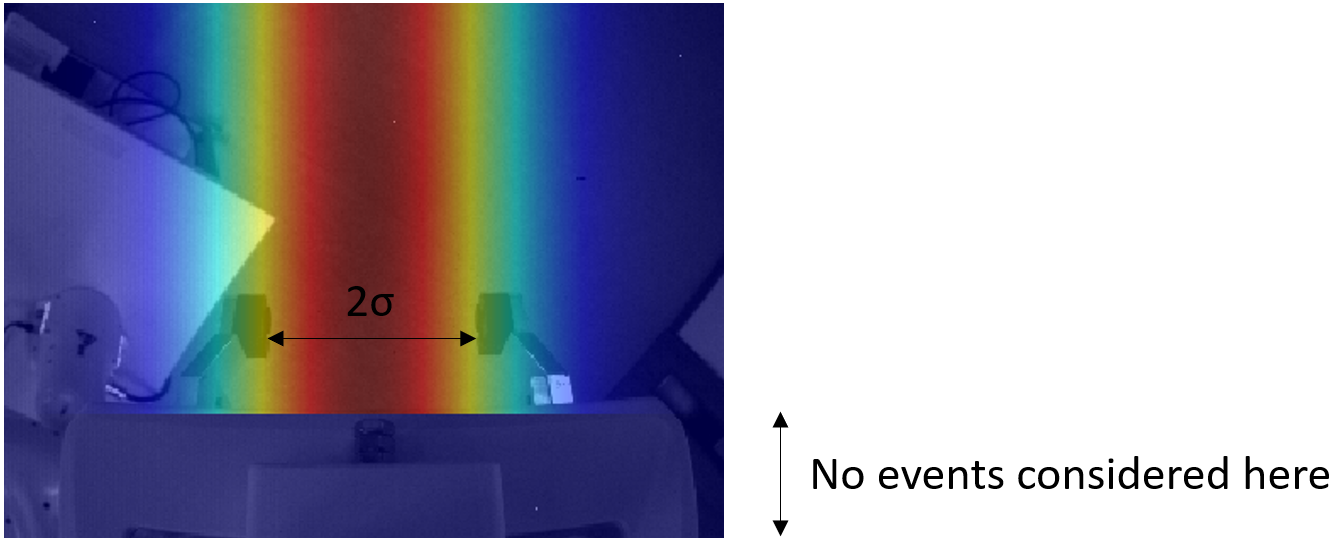
\includegraphics[width=0.8\textwidth]{resources/images/gaus_mask}
    \caption{Description of the weighted (Gaussian) mask.}\label{fig:gaus_mask}
\end{figure}

In ~\Cref{fig:fix_mask} some examples of Set 1 with this weighted mask have been depicted.

\begin{figure}[h]
    \centering
    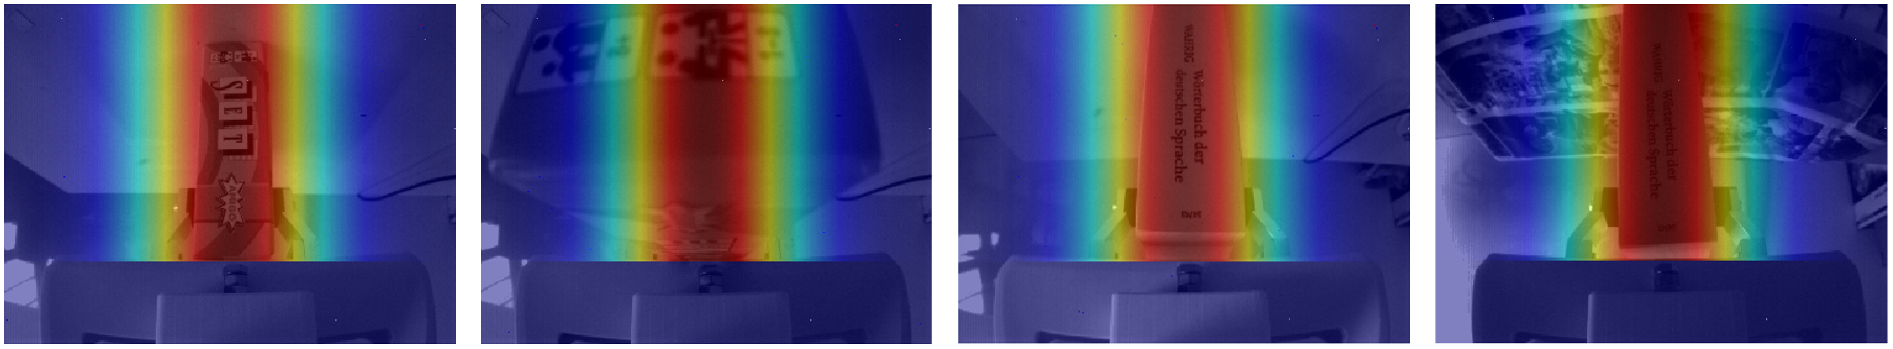
\includegraphics[width=\textwidth]{resources/images/fix_mask}
    \caption{Example initial frames of Set 1, with the weighted mask.}\label{fig:fix_mask}
\end{figure}

A comparison between the fixed RoI and weighted mask approach using some samples of Set 1, is reported in ~\Cref{fig:fix_mask_evr} and ~\Cref{fig:fix_mask_rat}. For the sequence of the box, where almost no slip occurs, we can observe how the weighted event rate is higher than the event rate inside the RoI, as events in the background are also weighted and taken into account. This produces an increase in the ratio values, having higher spikes. When the box slips, both event rates are nearly the same, as the object is mostly in the center of the image. In terms of the ratio, the peaks increase a bit. Overall, the slip detection can still be made, but with a higher threshold, around 0.6.\\

Considering the box with reverse grip, we can see how the weighted event rate is lower after than the RoI one, being significantly different from the event rate in the whole image. This happens as the RoI almost occupied the whole image, as shown in ~\Cref{fig:fix_roi}. Thanks to this adjustment in the event rate, the resulting ratio signal (using the weighted mask) allows us to detect two slips, with a threshold of 0.6 again, which is what happens in the sequence.\\

For book no. 1, in both cases the weighted event rate is higher than the RoI one, but specially in the highly textured table scenario, where many events are generated due to the background, which are weighted in the computation of the event rate. In terms of the ratio signal, the weighted mask shows better results, as using a threshold of 0.2, we can detect the slips, without influencing the highly textured background.

\begin{figure}[H]
    \centering
    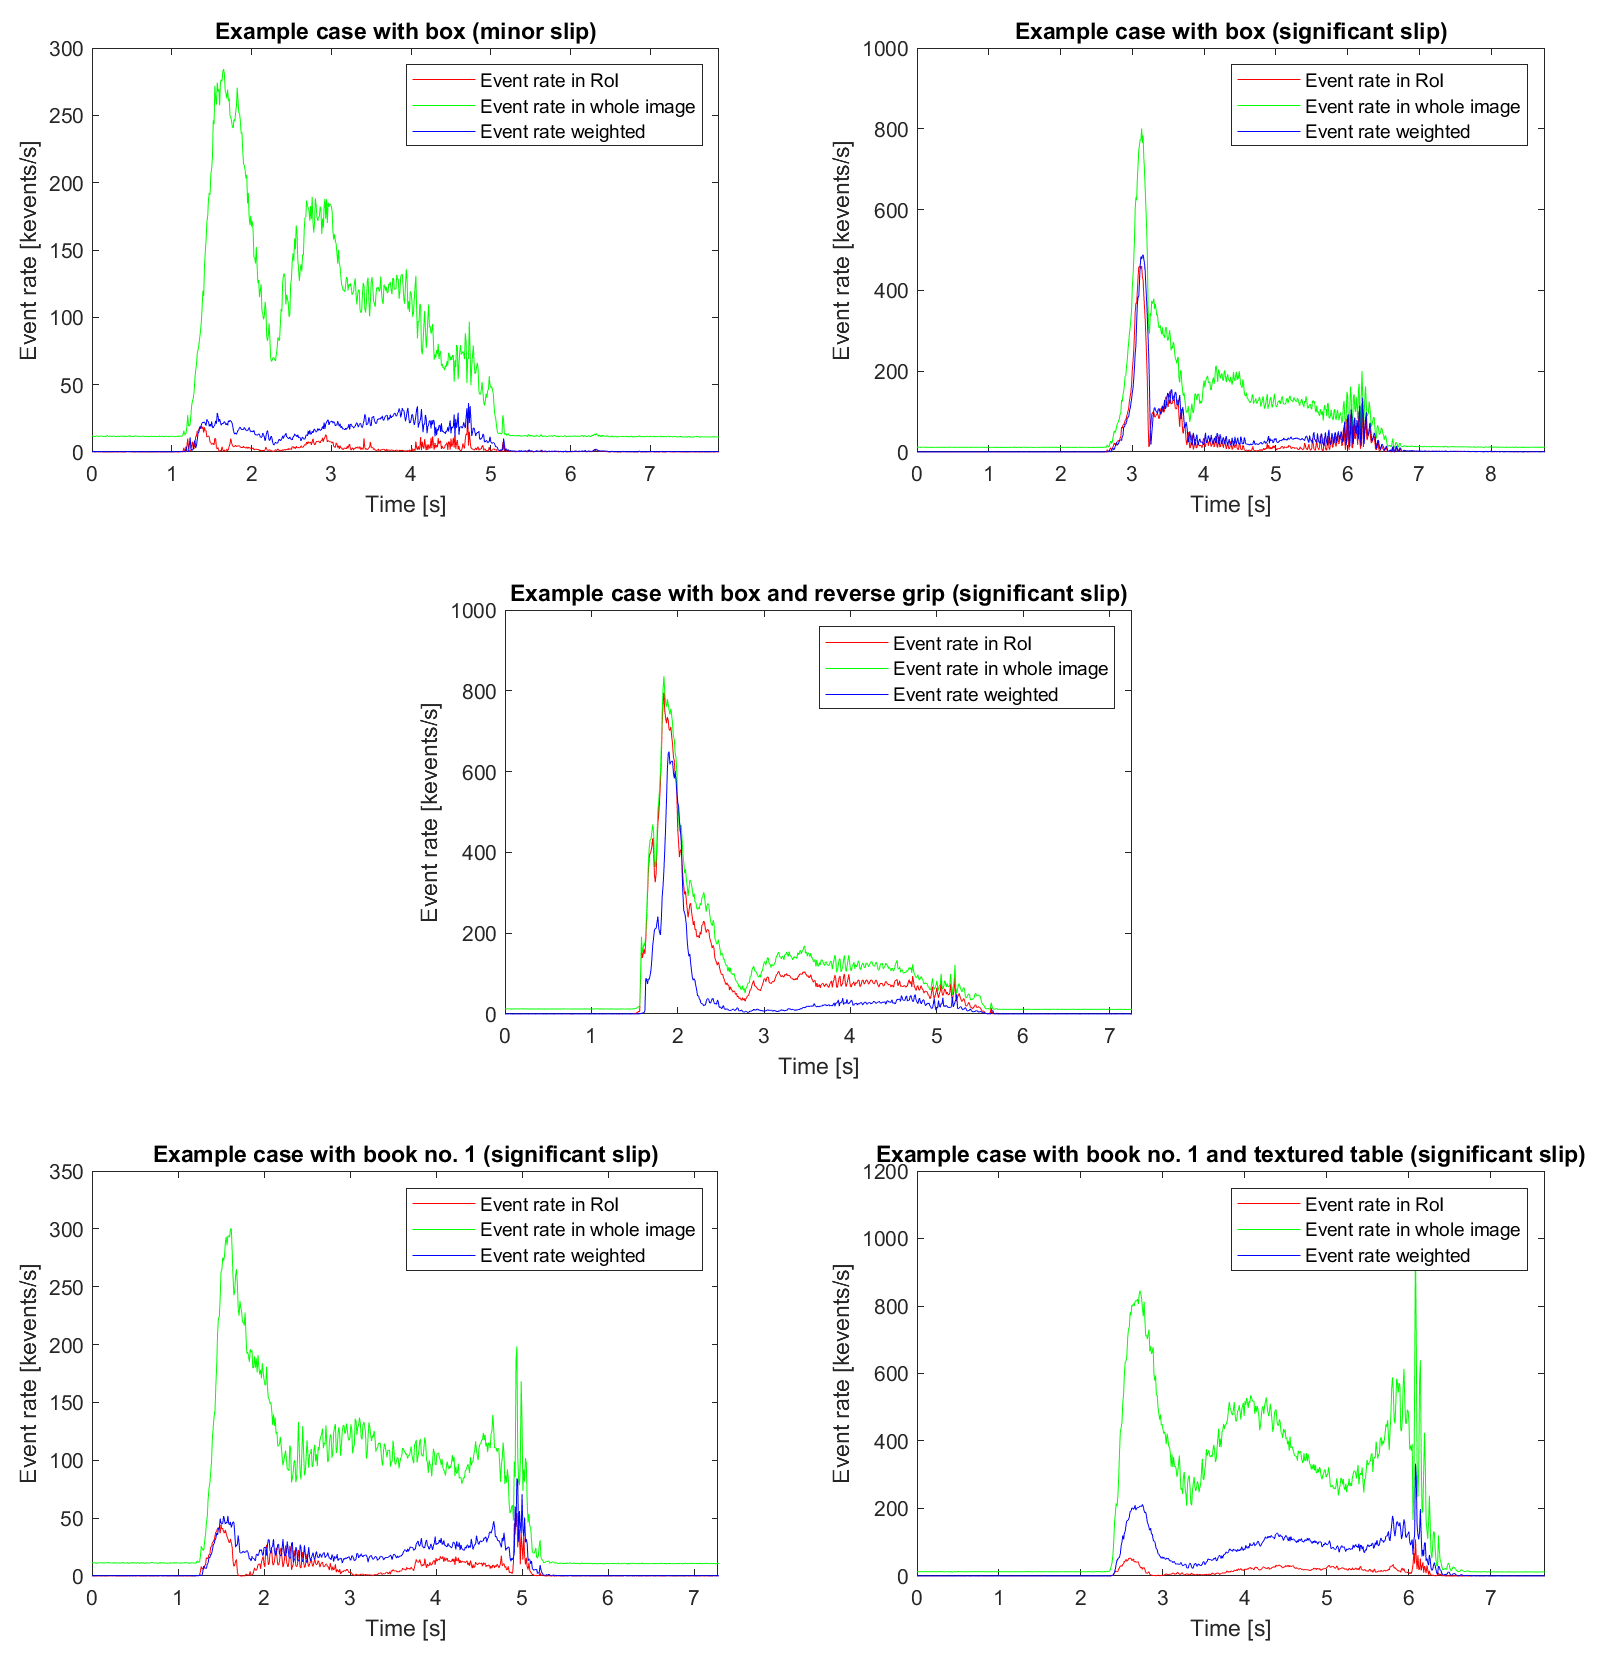
\includegraphics[width=\textwidth]{resources/images/fix_mask_evr}
    \caption{Event rate signals during some pick-and-place motions of Set 1 using the fixed RoI and weighted mask.}\label{fig:fix_mask_evr}
\end{figure}

In conclusion, this method solves some of the issues present with the fixed RoI approach:

\begin{itemize}
	\item The weighted mask does not need to be annotated for each scenario, as it is the same for all of them, using the prior of where the object will be grasped.
	\item For the cases where the object rotates a lot and the shape of it varies significantly from the camera's view, it works much better, as the ratio signal can be easily thresholded.
	\item It is more robust to changes in the background's texture.
\end{itemize}

However, the ratio threshold still depends on the object's texture, as for the box we would use 0.6, whereas for the book we would use only 0.2.

\begin{figure}[H]
    \centering
    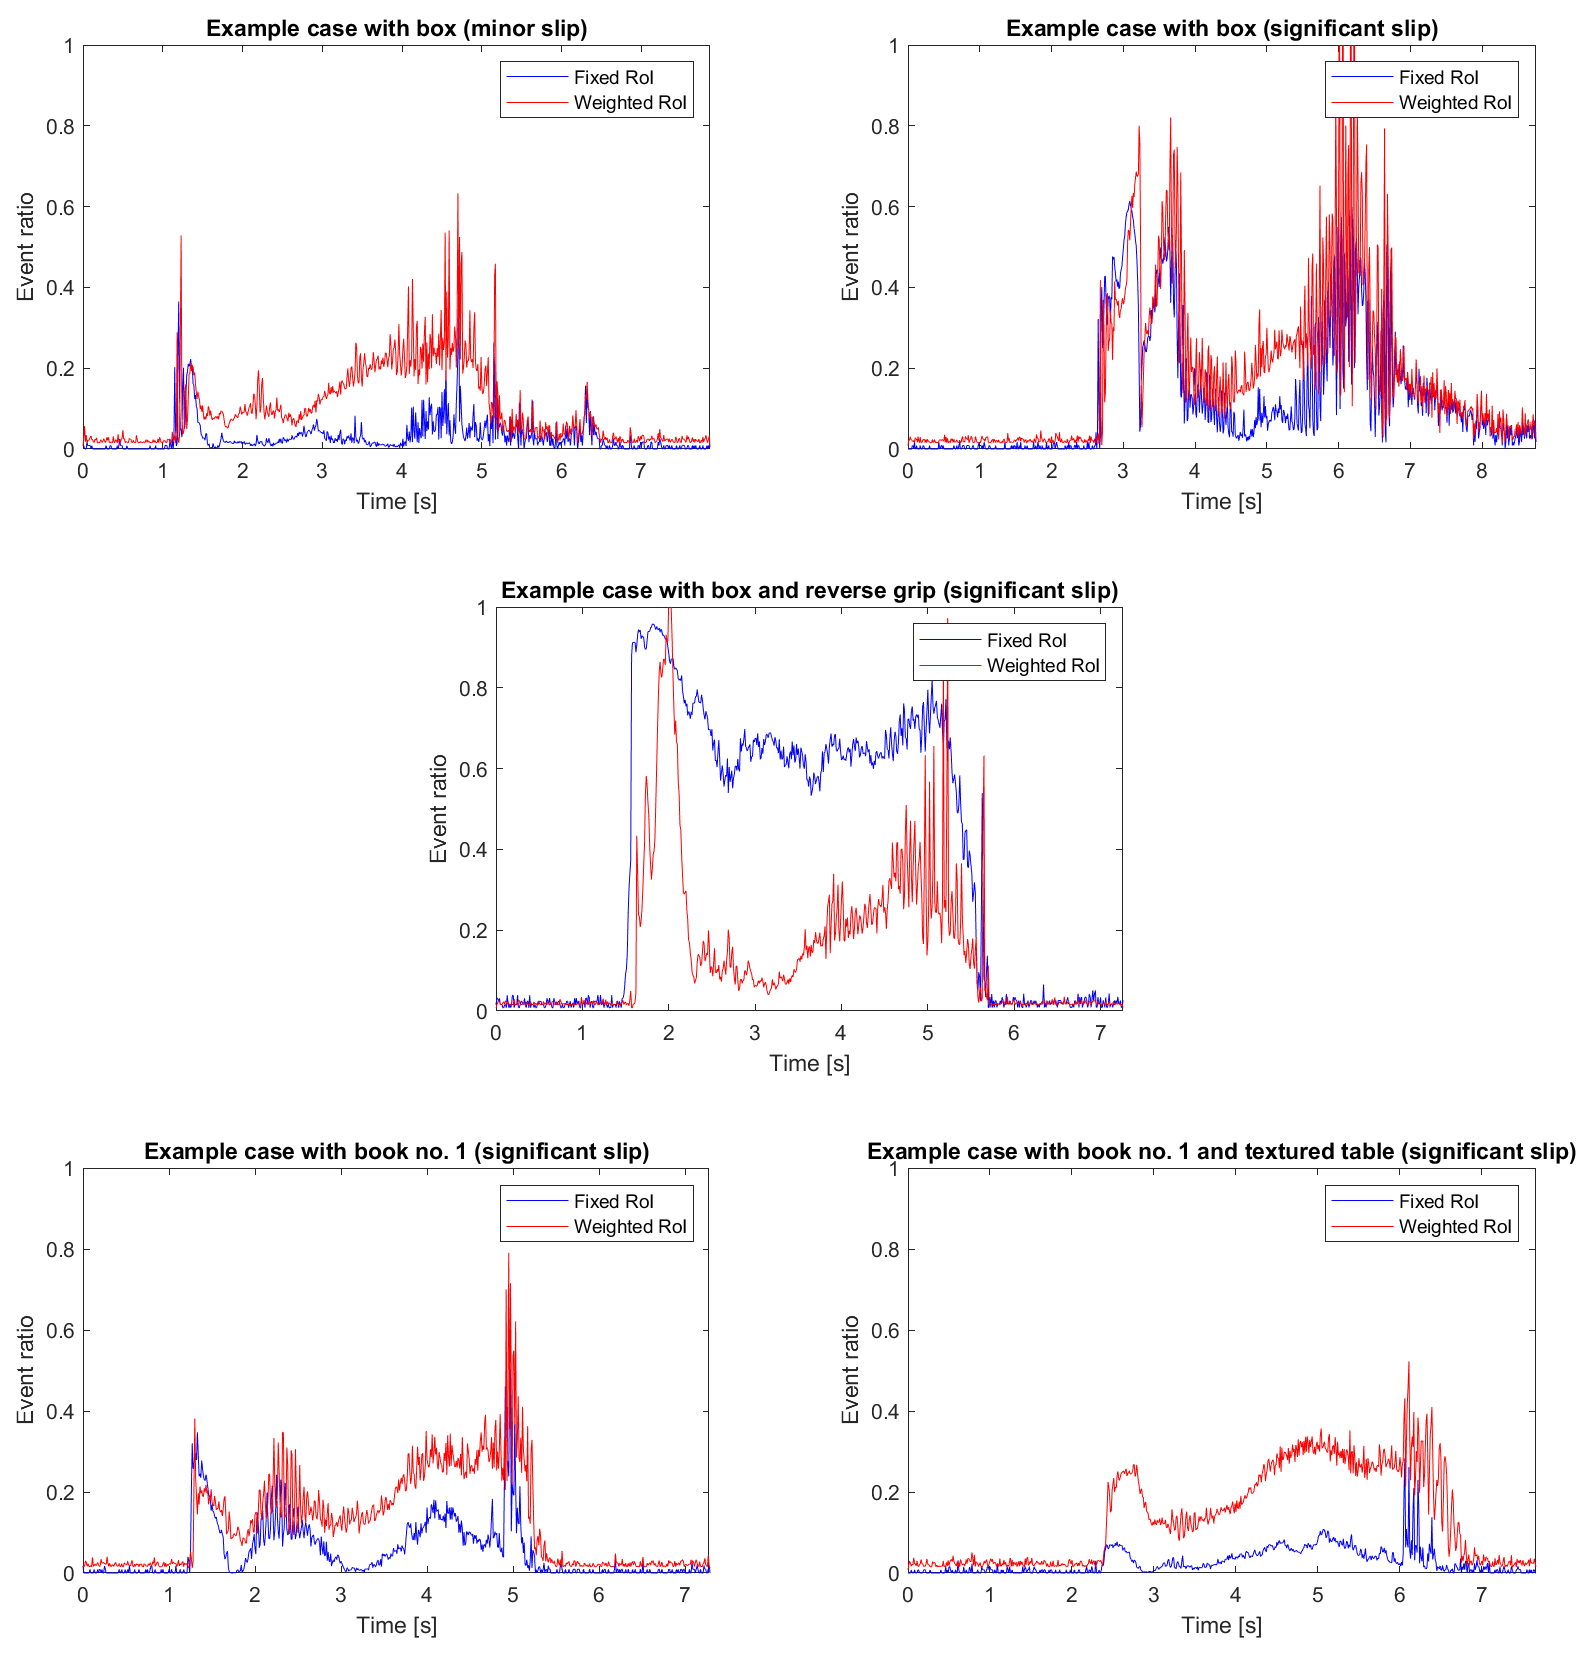
\includegraphics[width=\textwidth]{resources/images/fix_mask_rat}
    \caption{Ratio signals during some pick-and-place motions of Set 1 using the fixed RoI and weighted mask.}\label{fig:fix_mask_rat}
\end{figure}

\subsection{Results with Set 2 and variable mask}

Another way of dealing with the issues derived from using the fix RoI, is to compute a variable mask where the object is present. For instance, a detection algorithm can be run in the beginning and then the object can be tracked, however, this process can be really computationally expensive, which may be counterproductive when detecting slip using low latency sensors, such as the event-based camera. A naive approach to compute such mask is to record first a sequence without any object and then execute the same pick-and-place operation with different objects. After synchronizing both sequences, the grayscale frames can be subtracted and with that the object can be masked. Concretely, in ~\Cref{fig:var_mask_hb1}, the results of calculating the absolute difference between the sequence in ~\Cref{fig:set2_empty} and ~\Cref{fig:set2_case1} is reported. Then, a binary image is created by thresholding the absolute difference with a value of 50, meaning that any value above or equal than 50 is 1 and the rest 0. After that, some morphological operations are performed in order to get the final mask. Specifically, an opening operation is applied to get rid of the background and then a closing operation is done to fill the gaps in the masked object.

\begin{figure}[H]
    \centering
    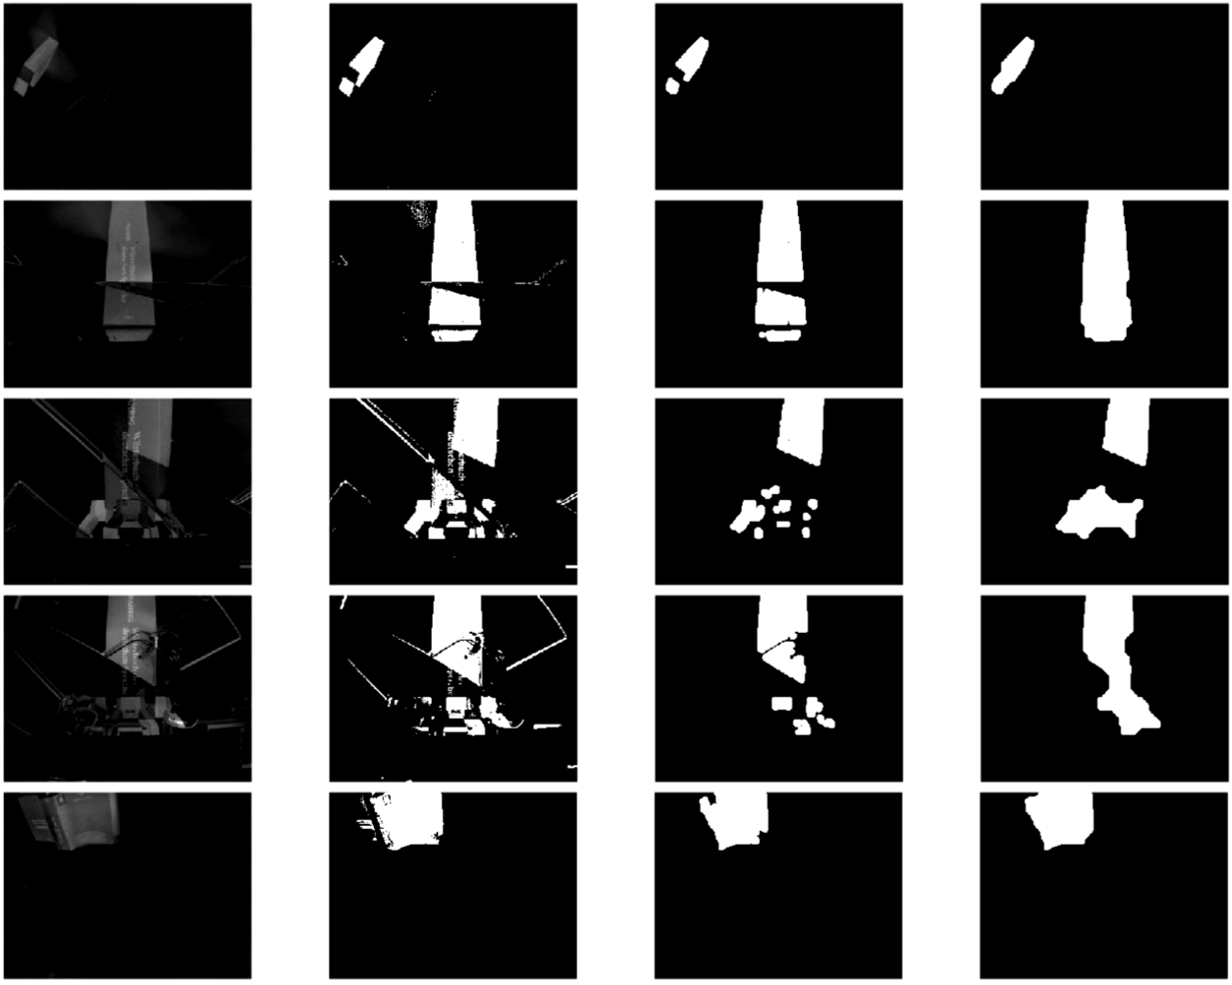
\includegraphics[width=\textwidth]{resources/images/var_mask_hb1}
    \caption{Sequence of images with the steps to generate the variable mask. The first column is the subtraction between the empty and with object sequence. The second is generated from the first by computing a binary image. Then, in the third, a opening operation is done and in the fourth a closing one is performed to generate the final mask.}\label{fig:var_mask_hb1}
\end{figure}

At a first, glance we can already realize that this method is quite brittle and present some clear disadvantages:

\begin{itemize}
	\item It is assumed that the background will not change between the initial empty sequence and the rest of experiments. So any change in the initial scene can affect the mask generation.
	\item If there are several objects to be picked (out of the scope of this thesis), all of them will be considered in the mask and not only the one picked.
	\item The object may have similar grayscale value as the background in some occasions and the subtraction may not include parts of the object (see  ~\Cref{fig:var_mask_hb1}).
\end{itemize}

It is worth mentioning that the grayscale frames are generated at 40 Hz, therefore, the mask is also updated at this frequency. In ~\Cref{fig:var_mask_hb1_no_slip_evr} and ~\Cref{fig:var_mask_hb1_no_slip_rat}, the results for a non-slip scenario with book no.1 are reported, where we can see that both the event rate and ratio signals are low. Notice that the signals calculated through the weighted fix mask are always higher than the ones from the variable mask, as for the former all the events in the scene are taken into account with the corresponding weight. Note that the signals are only shown during the manipulation phase of the object, where slip should be detected.\\

In contrast, for the slip scenario, the results are shown in ~\Cref{fig:var_mask_hb1_slip_evr} and ~\Cref{fig:var_mask_hb1_slip_rat}. In this case, the ratio signal can be thresholded in both cases to detect the initial peak, corresponding to the main slip, and the second one, which is a slight slip.\\

For book no. 2, in ~\Cref{fig:var_mask_hb2_no_slip_evr} and ~\Cref{fig:var_mask_hb2_no_slip_rat} the results for the non-slip case are reported. By looking at the event rate signals one cannot appreciate any slip, however, the ratio signals present a peak in the beginning which would cause a false positive in terms of slip detection. For the slip case (see ~\Cref{fig:var_mask_hb2_slip_evr} and ~\Cref{fig:var_mask_hb2_slip_rat}), the event rate has an initial and final peak, coinciding with the two slips present in the sequence, but looking at the ratio signal no clear differences can be observed compared to the non-slip case. Hence, this method fails to detect slip in these two sequences.

\begin{figure}[H]
    \centering
    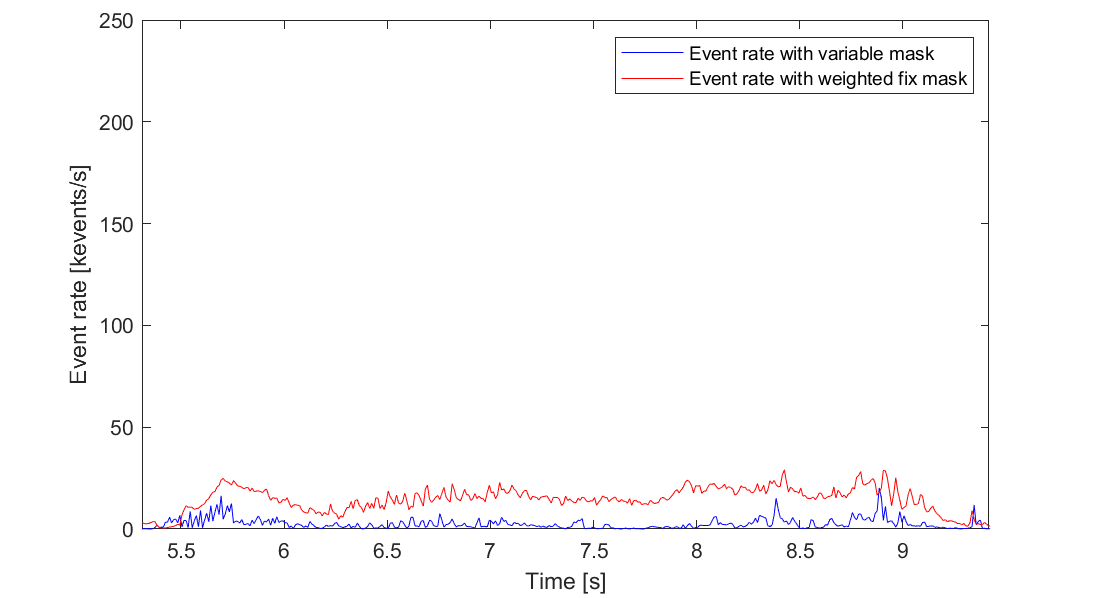
\includegraphics[width=0.86\textwidth]{resources/images/var_mask_hb1_no_slip_evr}
    \caption{Event rate signals of ~\Cref{fig:set2_case1} using the weighted fix and variable mask.}\label{fig:var_mask_hb1_no_slip_evr}
\end{figure}

\begin{figure}[H]
    \centering
    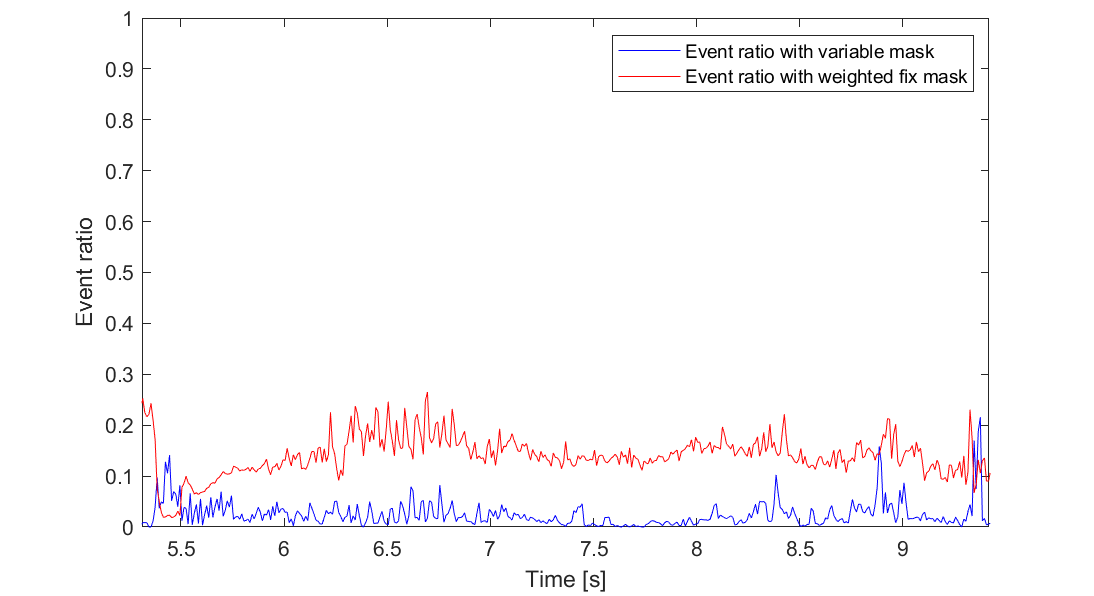
\includegraphics[width=0.86\textwidth]{resources/images/var_mask_hb1_no_slip_rat}
    \caption{Ratio signals of ~\Cref{fig:set2_case1} using the weighted fix and variable mask.}\label{fig:var_mask_hb1_no_slip_rat}
\end{figure}

\begin{figure}[H]
    \centering
    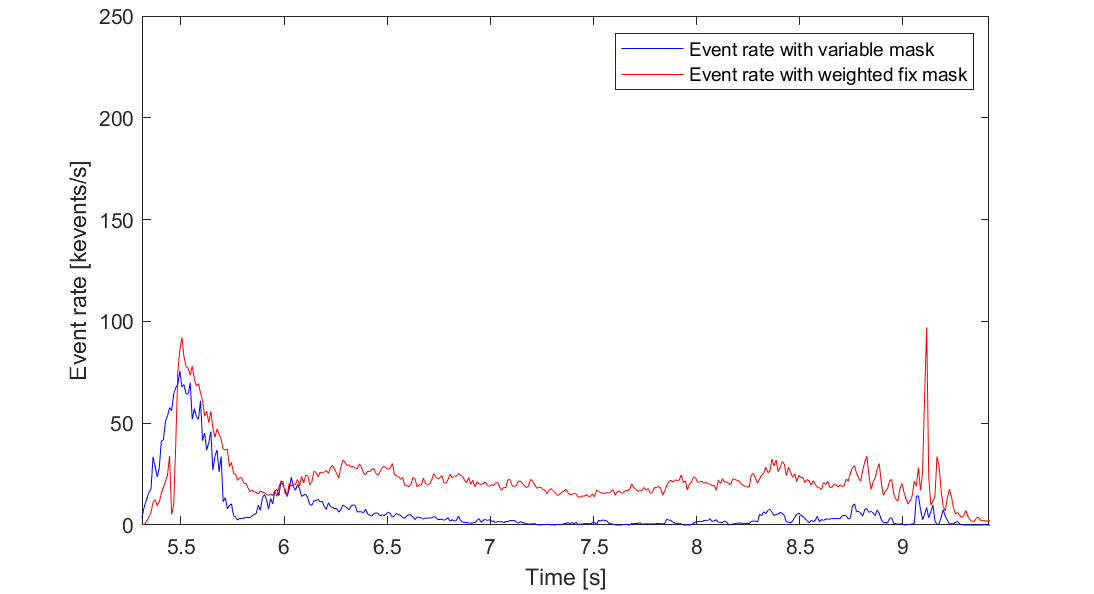
\includegraphics[width=0.86\textwidth]{resources/images/var_mask_hb1_slip_evr}
    \caption{Event rate signals of ~\Cref{fig:set2_case2} using the weighted fix and variable mask.}\label{fig:var_mask_hb1_slip_evr}
\end{figure}

\begin{figure}[H]
    \centering
    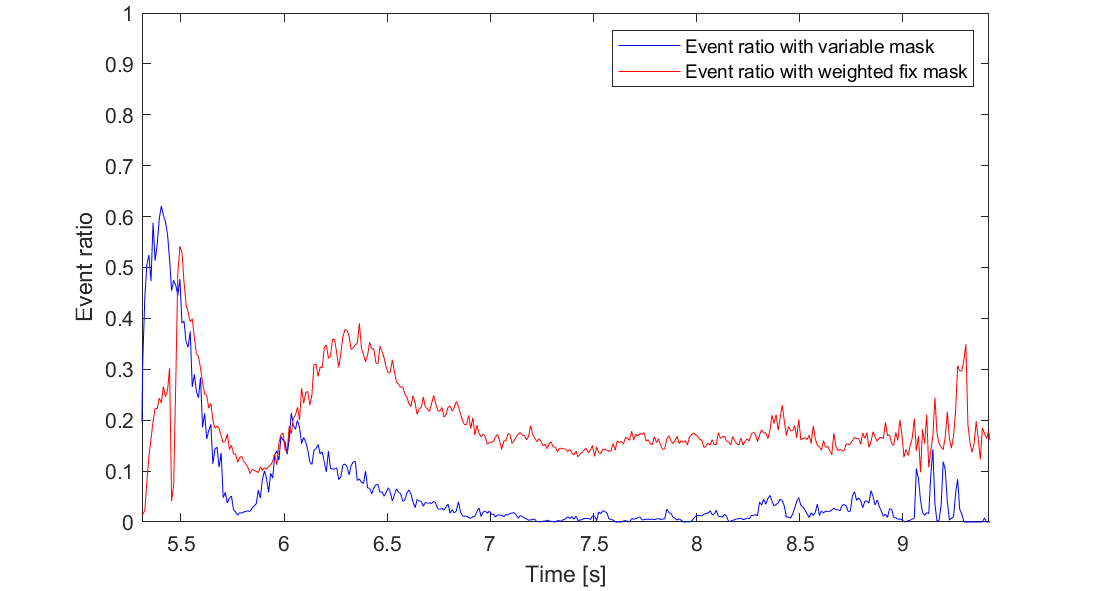
\includegraphics[width=0.86\textwidth]{resources/images/var_mask_hb1_slip_rat}
    \caption{Ratio signals of ~\Cref{fig:set2_case2} using the weighted fix and variable mask.}\label{fig:var_mask_hb1_slip_rat}
\end{figure}

\begin{figure}[H]
    \centering
    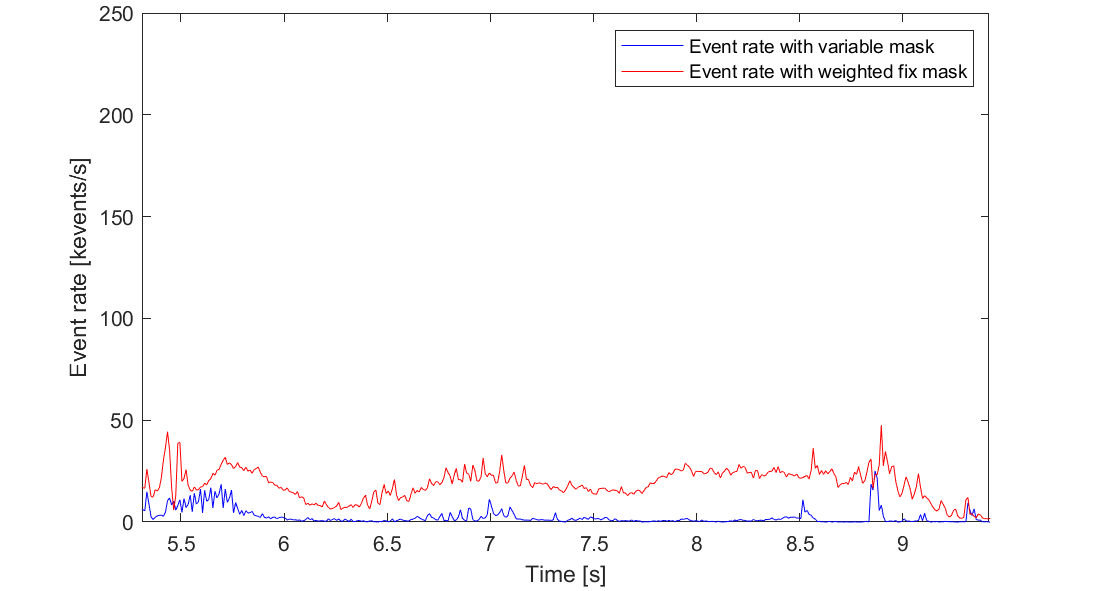
\includegraphics[width=0.86\textwidth]{resources/images/var_mask_hb2_no_slip_evr}
    \caption{Event rate signals of ~\Cref{fig:set2_case4} using the weighted fix and variable mask.}\label{fig:var_mask_hb2_no_slip_evr}
\end{figure}

\begin{figure}[H]
    \centering
    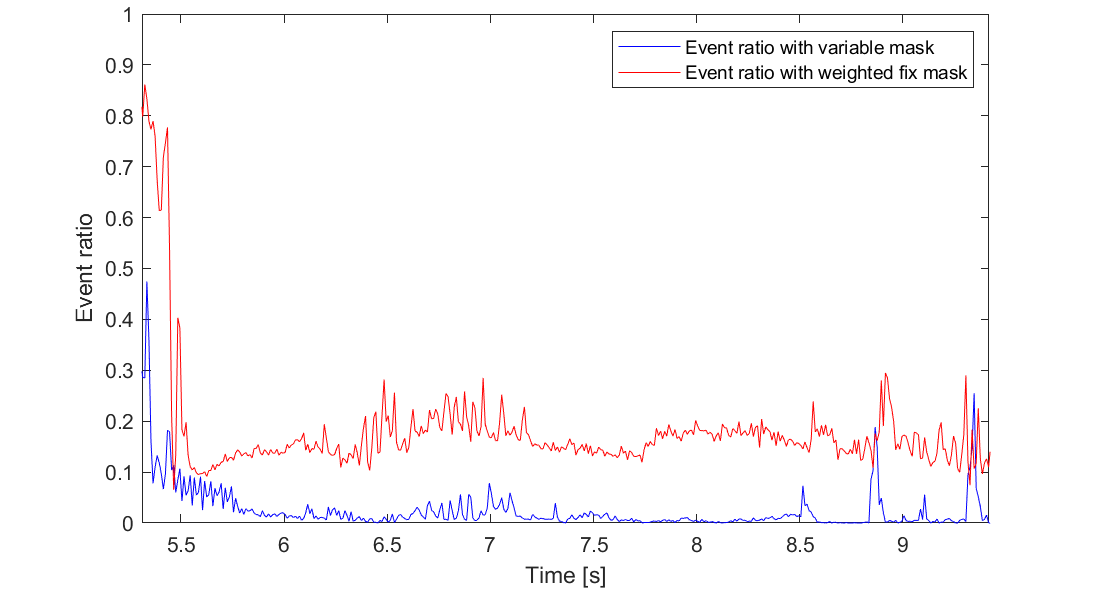
\includegraphics[width=0.86\textwidth]{resources/images/var_mask_hb2_no_slip_rat}
    \caption{Ratio signals of ~\Cref{fig:set2_case4} using the weighted fix and variable mask.}\label{fig:var_mask_hb2_no_slip_rat}
\end{figure}

\begin{figure}[H]
    \centering
    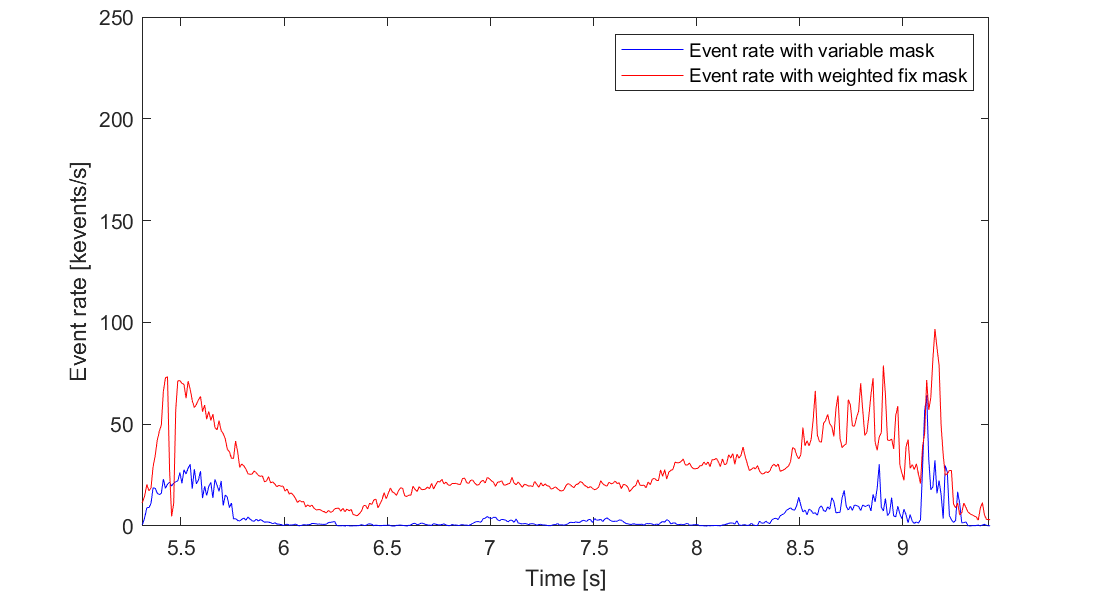
\includegraphics[width=0.86\textwidth]{resources/images/var_mask_hb2_slip_evr}
    \caption{Event rate signals of ~\Cref{fig:set2_case5} using the weighted fix and variable mask.}\label{fig:var_mask_hb2_slip_evr}
\end{figure}

\begin{figure}[H]
    \centering
    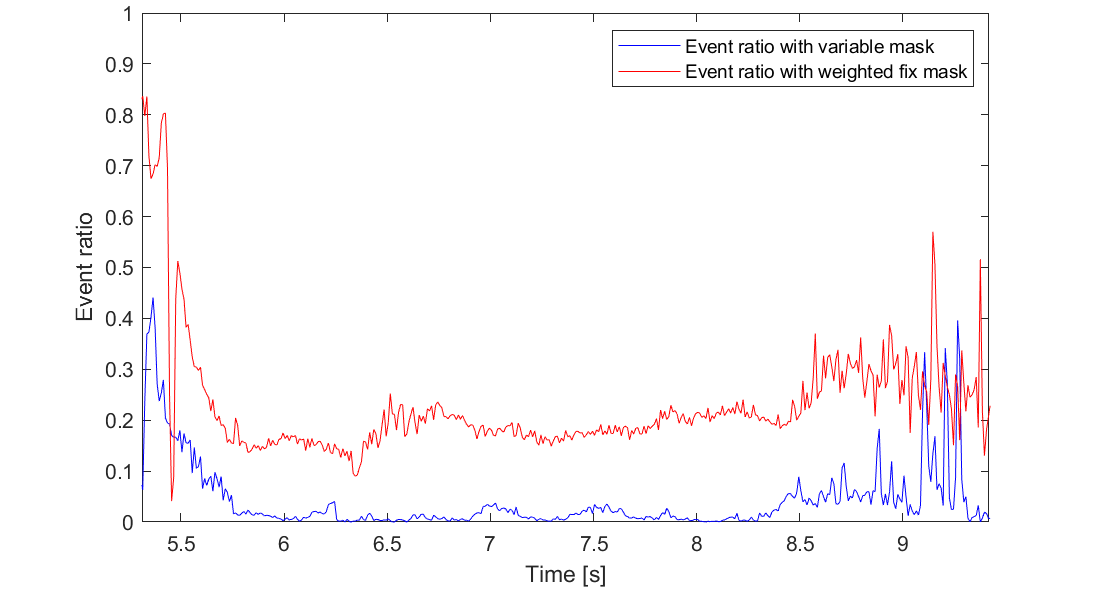
\includegraphics[width=0.86\textwidth]{resources/images/var_mask_hb2_slip_rat}
    \caption{Ratio signals of ~\Cref{fig:set2_case5} using the weighted fix and variable mask.}\label{fig:var_mask_hb2_slip_rat}
\end{figure}

In conclusion, the weighted fix mask and the variable one, present similar results, where the former presents generally higher values in the event rate and ratio signals. Also, the variable mask method requires of extra computations to get this changing mask, which comes with the cost of being highly dependent on the background and the changes that may occur between the initial empty sequence compared to the following pick-and-place motions.

\section{Optical flow analysis}

\subsection{Introduction}

By looking at the moving edges in the event images, the motion of the object can be distinguished. Also, the event rate gives a notion of how the velocity of the object increases. However, for this purpose, per pixel velocity in each axis of the image may be more suitable. Actually, the motion estimation can be done through optical flow, which is the pattern of apparent motion of objects, surfaces and edges in a visual scene caused by the relative motion between an observer and a scene.\\

Concretely, we use EV-FlowNet ~\cite{evflownet}, a self-supervised deep learning pipeline for optical flow estimation for event-based cameras. 

\subsection{Results with Gelsight dataset}

First, optical flow was analyzed with the Gelsight dataset ~\cite{gelsight2018}. The EV-FlowNet algorithm outputs the pixel-wise velocities in \textit{x} and \textit{y}-axis of the image, given the grayscale frames and the events. These velocities are given at 40 Hz, which corresponds to the rate at which the grayscale images are provided.\\

At each instant, the absolute mean velocity in each direction is computed (for all the pixels in the image). In addition, the pixels where the velocity norm is nearly zero (considered as any value lower than 0.01) are removed from the mean, in order to have a variation in the mean when there is motion coming from the object. In ~\Cref{fig:gelsight_of}, the absolute mean velocities in \textit{x} and \textit{y} directions for 4 samples of object 1 have been reported. Due to the EV-FlowNet algorithm, the estimation is only provided until 0.6 s, instead of reaching the total duration (1 s) of the sequence.\\

During a perfect grasp, as happens in the sequence ~\Cref{fig:gelsight_case1}, with a gripper width of 66.6 mm, the velocities are nearly zero during the whole sequence.\\

For the sequences represented in ~\Cref{fig:gelsight_case2} and ~\Cref{fig:gelsight_case3}, with a gripper width of 67.2 and 67.3 mm respectively, there is a slight slip in the beginning that stops. This behavior can also be analyzed by looking at the velocities, having a small peak in the velocities for a width of 67.2 mm and a higher peak for 67.3 mm. However, the later width produces a failure in the grasping just in the end, which cannot be detected by looking at the velocities, as the data is cropped to 0.6 s.\\

Finally, in a scenario where the gripper fails to grasp the object, as happened in ~\Cref{fig:gelsight_case4}, with a gripper width of 67.5 mm, the velocities are high during the whole sequence, as the object stays in the table while the gripper and the attached camera move away from it.

\begin{figure}[h]
    \centering
    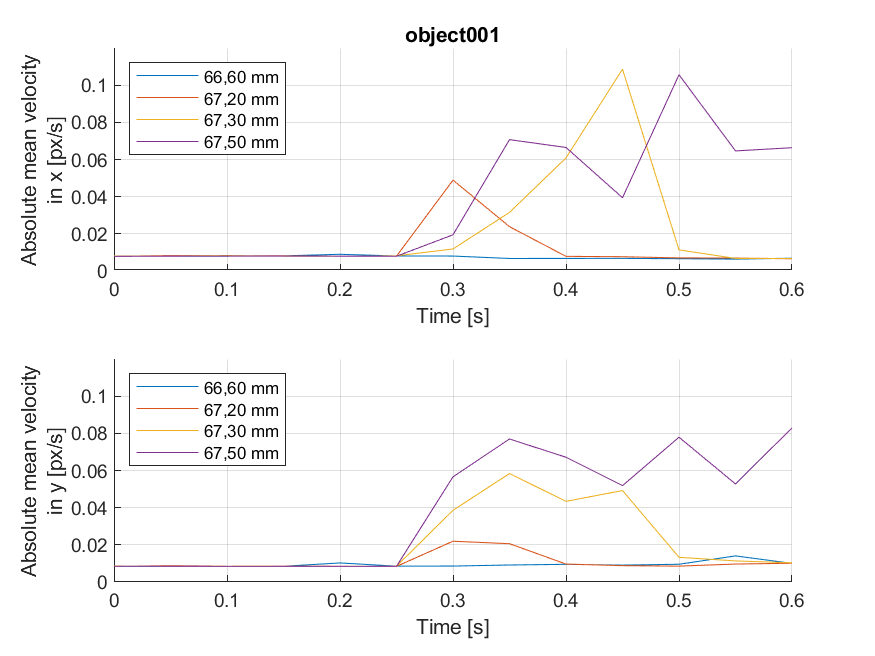
\includegraphics[width=\textwidth]{resources/images/gelsight_of}
    \caption{Comparison of the absolute mean velocities' evolution in the whole image for 4 samples of object 1 from the dataset in ~\cite{gelsight2018}.}\label{fig:gelsight_of}
\end{figure}

\subsection{Results with Set 1}

The output from optical flow can be coded into HSV (Hue Saturation and Value) format for visualizing the data. Concretely, the hue encodes the angle of the velocity, the saturation represents the norm of it and the value is set at its maximum always. In ~\Cref{fig:OF_angle} the encoding of the norm and angle are depicted, where the angles show different colors and the norm regulates their intensity.\\

\begin{figure}[h]
    \centering
    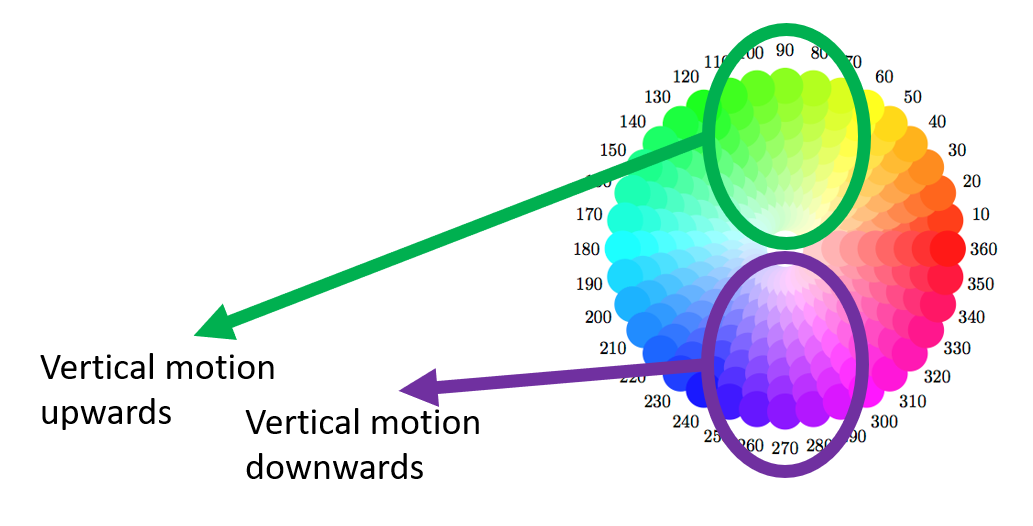
\includegraphics[width=0.8\textwidth]{resources/images/OF_angle}
    \caption{Colomap resulting from the encoding of the norm and angle of the optical flow velocities.}\label{fig:OF_angle}
\end{figure}

In ~\Cref{fig:OF_set_no_slip}, the motion estimation for a non-slip case is shown. As one may notice, there is no motion in the center of the image, precisely where the object is. Instead, in ~\Cref{fig:OF_set_slip}, in the first two rows the motion of the object can be clearly seen, coinciding with the slips. First, a rotation occurs in one direction, such that the object moves downwards in the image plane. The estimated motion shown for this case is represented by the colors pink, purple and dark blue, which precisely correspond to the observed vertical motion downwards, as indicated in ~\Cref{fig:OF_angle}. On the contrary, the second rotation happens inn the opposite direction, such that the object moves upwards in the image plane. The estimated motion shown for this case is represented by the colors green and yellow, which precisely correspond to the observed vertical motion upwards, as indicated in ~\Cref{fig:OF_angle}.

\begin{figure}[H]
    \centering
    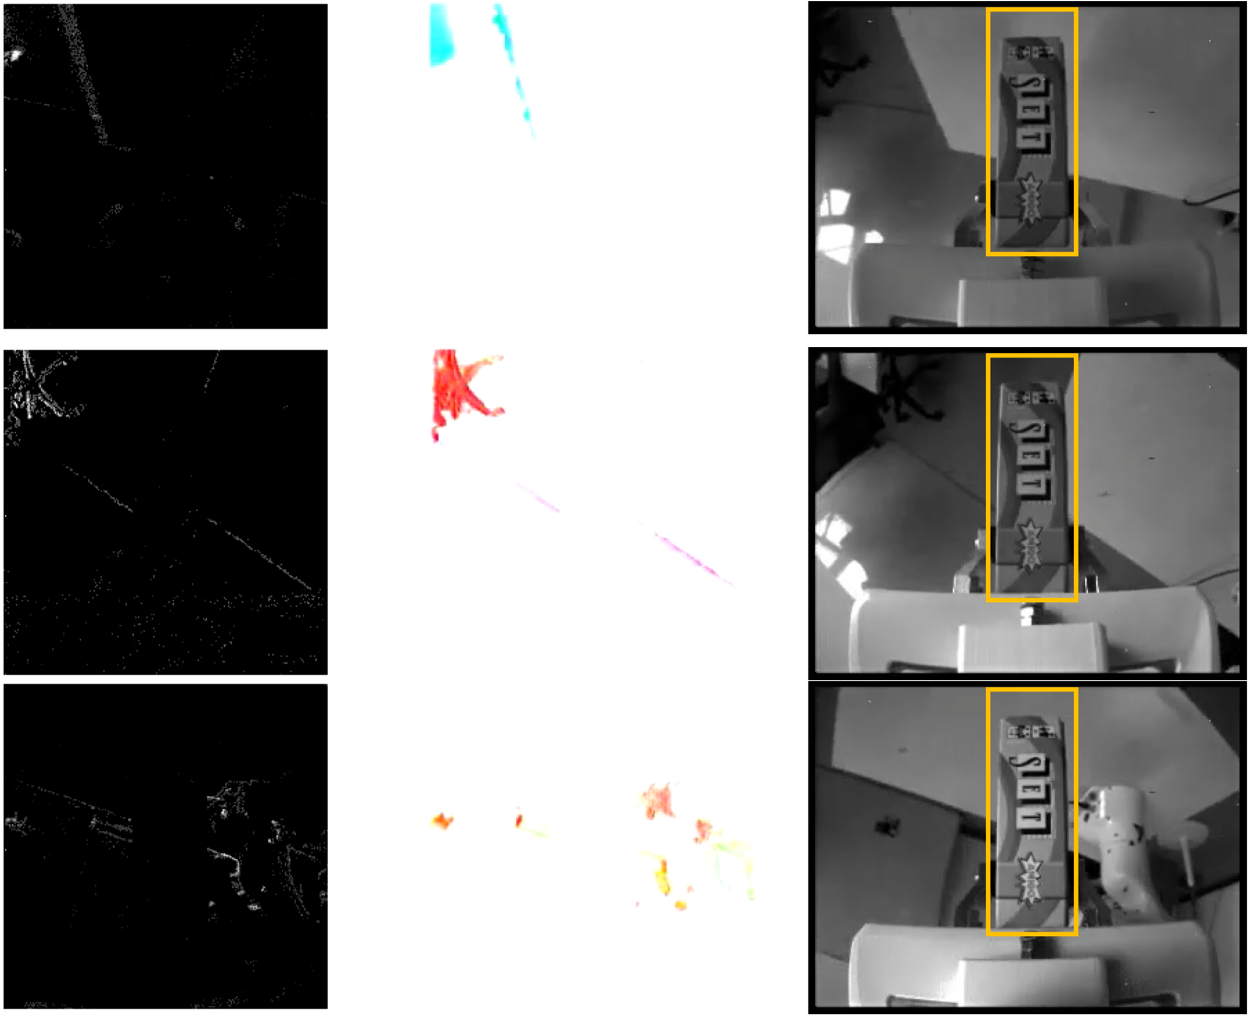
\includegraphics[width=\textwidth]{resources/images/OF_set_no_slip}
    \caption{Event images (first column), motion flow estimation using optical flow (second column) and grayscale frames (third column) for the sequence in ~\Cref{fig:set1_case1}.}\label{fig:OF_set_no_slip}
\end{figure}

\begin{figure}[H]
    \centering
    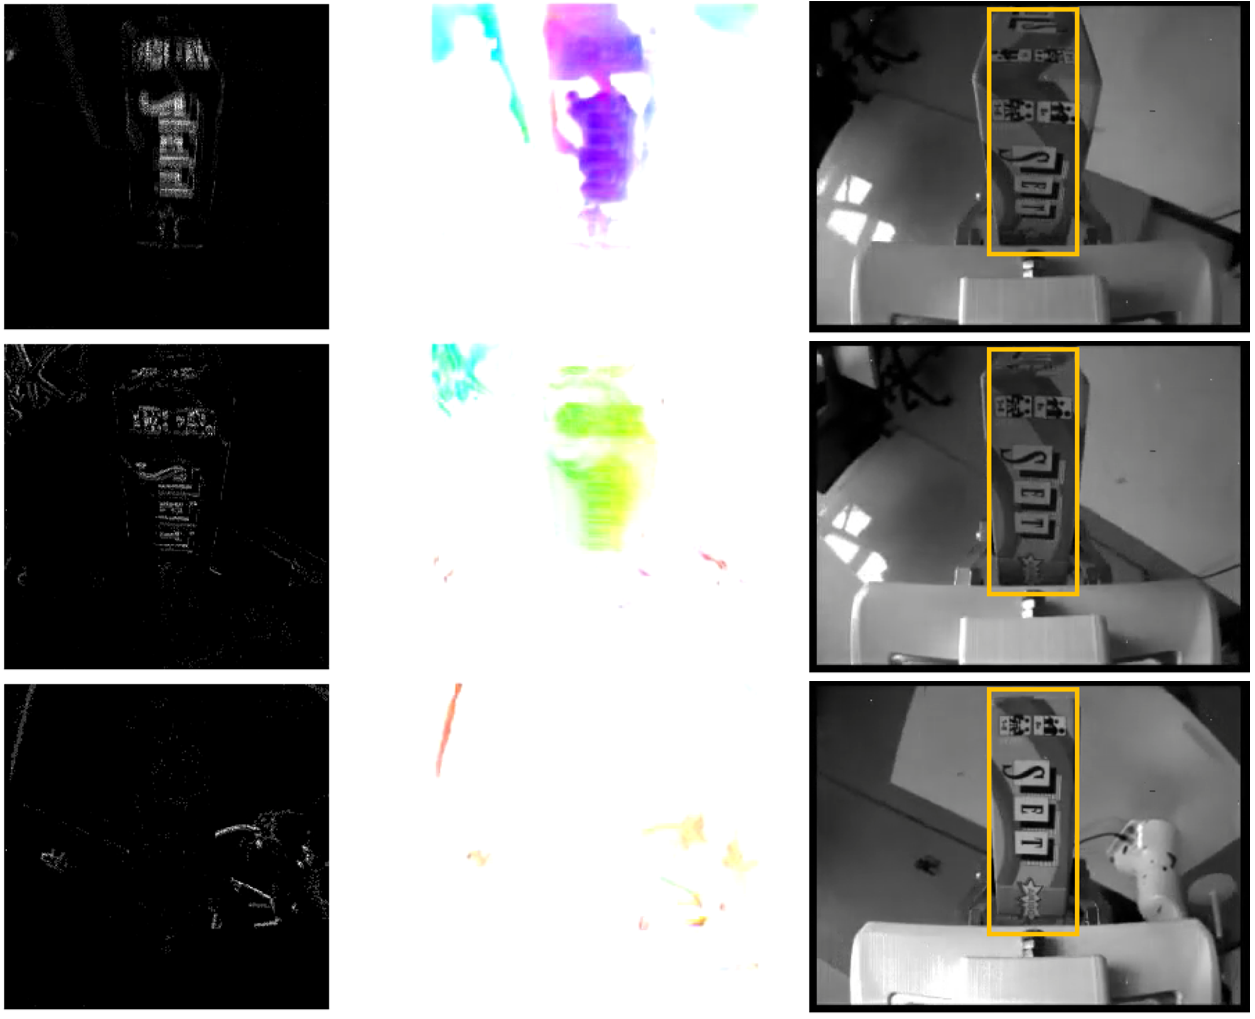
\includegraphics[width=\textwidth]{resources/images/OF_set_slip}
    \caption{Event images (first column), motion flow estimation using optical flow (second column) and grayscale frames (third column) for the sequence in ~\Cref{fig:set1_case2}.}\label{fig:OF_set_slip}
\end{figure}

Moreover, for the reverse grip, where the motion is quite abrupt, the resulting motion estimation for a concrete instant is depicted in ~\Cref{fig:OF_set_rev}. Here, there is a predominant vertical motion upwards, indicated by the green and yellow colors. However, in the left and right edges of the object, the pixels are moving towards the center, producing a horizontal motion in them, which is depicted with the red and cyan colors.

\begin{figure}[H]
    \centering
    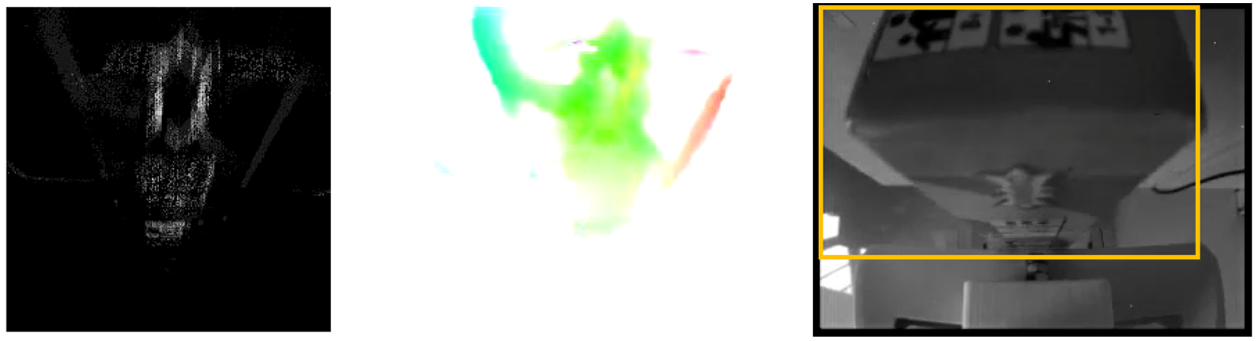
\includegraphics[width=\textwidth]{resources/images/OF_set_rev}
    \caption{Event images (first column), motion flow estimation using optical flow (second column) and grayscale frames (third column) for the sequence in ~\Cref{fig:set1_case6}.}\label{fig:OF_set_rev}
\end{figure}

Using book no. 1, as depicted in ~\Cref{fig:OF_hb1}, we can also detect vertical motion with green and purple colors. However, if the same experiment is repeated with a highly textured background, as reported in ~\Cref{fig:OF_hb1_tt}, the motion estimated for the background is predominant and the one for the object during slip is interpolated from the background, regarding the angle of the velocities.

\begin{figure}[H]
    \centering
    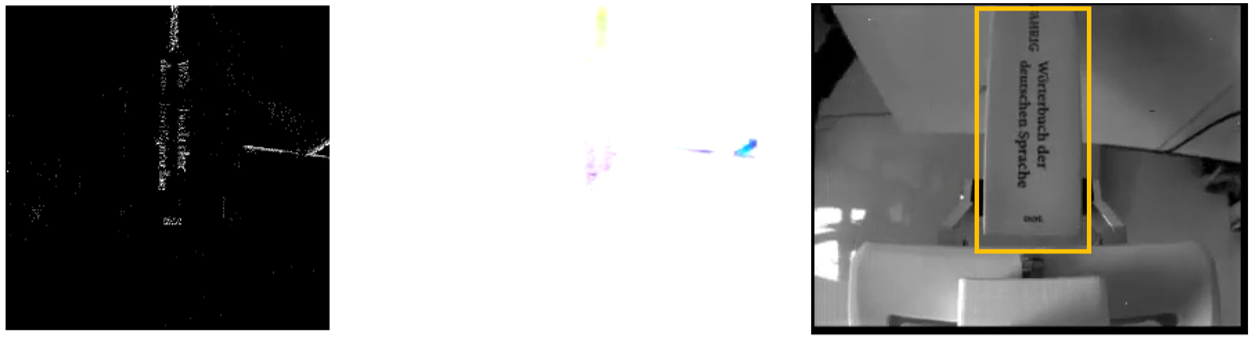
\includegraphics[width=\textwidth]{resources/images/OF_hb1}
    \caption{Event images (first column), motion flow estimation using optical flow (second column) and grayscale frames (third column) for the sequence in ~\Cref{fig:set1_case3}.}\label{fig:OF_hb1}
\end{figure}

\begin{figure}[H]
    \centering
    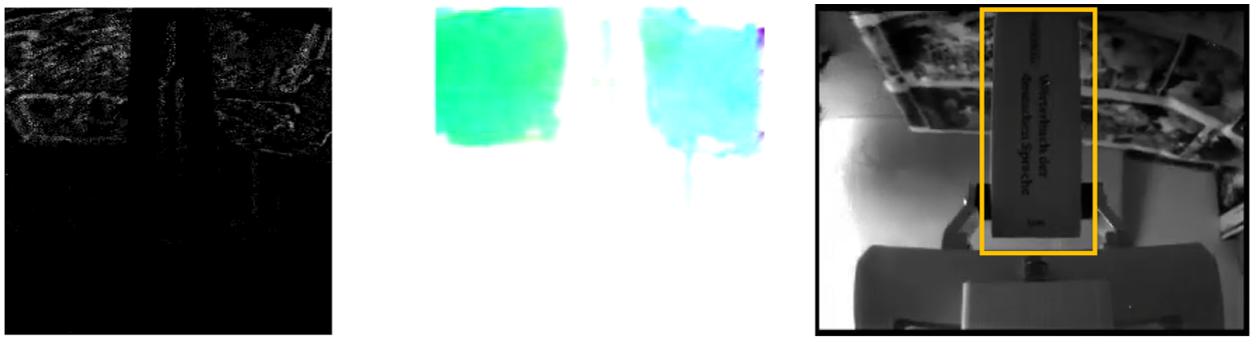
\includegraphics[width=\textwidth]{resources/images/OF_hb1_tt}
    \caption{Event images (first column), motion flow estimation using optical flow (second column) and grayscale frames (third column) for the sequence in ~\Cref{fig:set1_case7}.}\label{fig:OF_hb1_tt}
\end{figure}

These motion flow plots are informative visually, but not directly useful for slip detection. To this end, the absolute mean velocity for each axis is computed, as previously described. The differences with the Gelsight dataset are that now the object and the background motion should be somehow separated and we are interested in the vertical motion, as all examples suffer from the described rotational slip. To focus on the motion produced by the object, we can use the fixed RoI approach or the weighted mask one, which were used for generating the event rate and ratio signals.\\

First, for a non-slip case, as reported in ~\Cref{fig:OF_comparison_set_no_slip}, there is a nearly zero velocity in the vertical axis (\textit{y}), which would indicate that there is no vertical motion in the object, meaning no slip occurred. For the horizontal axis (\textit{x}), we can see a peak in the beginning, due to the background, which is not perfectly separated from the object in both cases. In contrast, in a slip example, shown in ~\Cref{fig:OF_comparison_set}, there are two evident peaks in the vertical velocity, which correspond to the two rotational slips present in the sequence. Concretely, for the weighted mask approach the signal presents higher values. Moreover, in the reverse grip example (see ~\Cref{fig:OF_comparison_set_rev}), the vertical motion again shows how there is a slip in the beginning of the experiment. As previously pointed out, in this example, there is also horizontal motion in some parts of the object, which produces as well a peak in the velocity in \textit{x}.\\

For the book experiment, as observed in ~\Cref{fig:OF_comparison_hb1}, the fixed RoI approach presents two small peaks, one in the beginning and one in the end, due to the two small slips present in the experiment. However, for the weighted mask approach, there are several spikes in the middle of the sequence, producing false positives, which may be due to the background's motion. 

\begin{figure}[H]
    \centering
    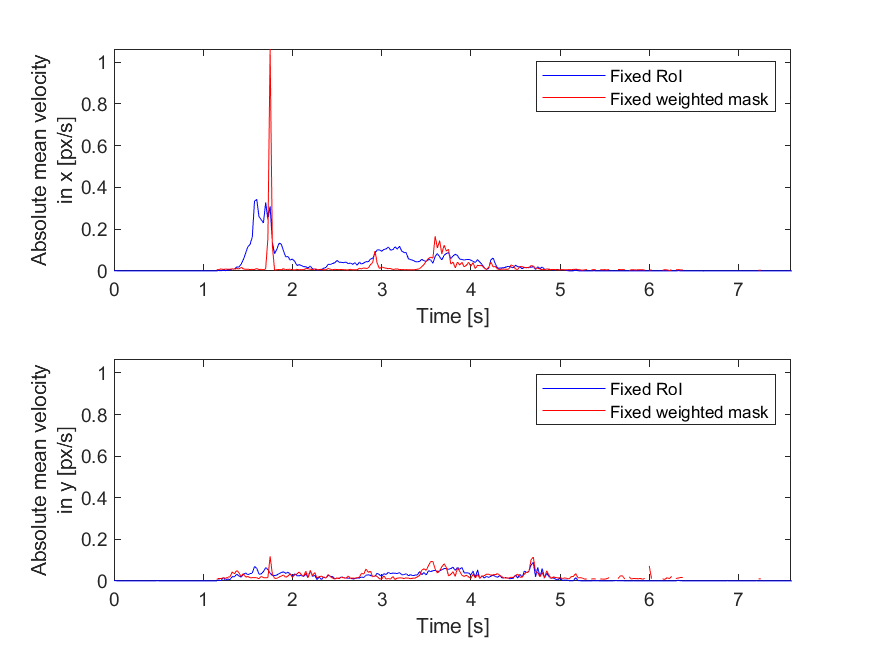
\includegraphics[width=0.95\textwidth]{resources/images/OF_comparison_set_no_slip}
    \caption{Comparison of the absolute mean velocities' evolution in the whole image for the sequence in ~\Cref{fig:set1_case1}.}\label{fig:OF_comparison_set_no_slip}
\end{figure}

\begin{figure}[H]
    \centering
    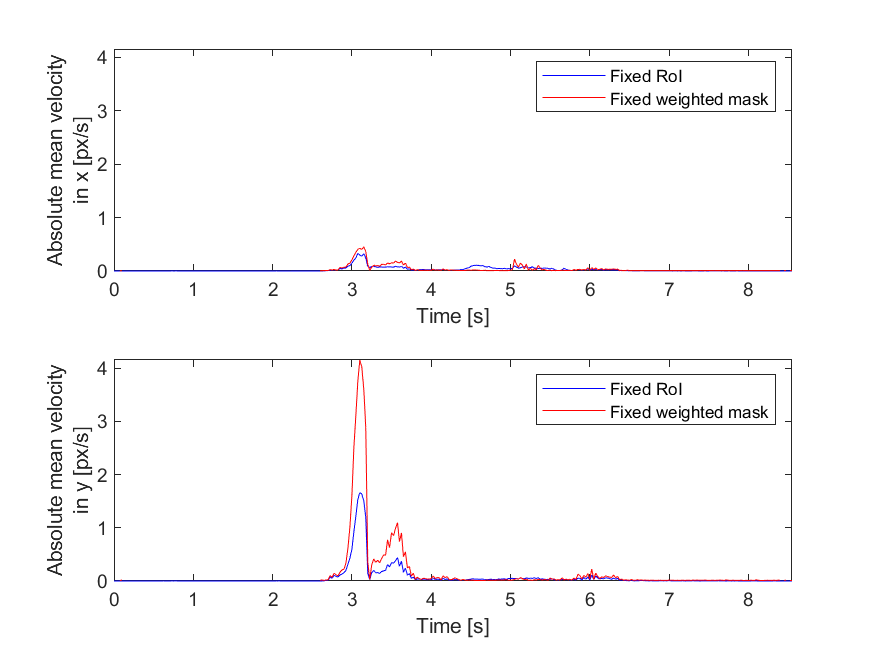
\includegraphics[width=0.95\textwidth]{resources/images/OF_comparison_set}
    \caption{Comparison of the absolute mean velocities' evolution in the whole image for the sequence in ~\Cref{fig:set1_case2}.}\label{fig:OF_comparison_set}
\end{figure}

\begin{figure}[H]
    \centering
    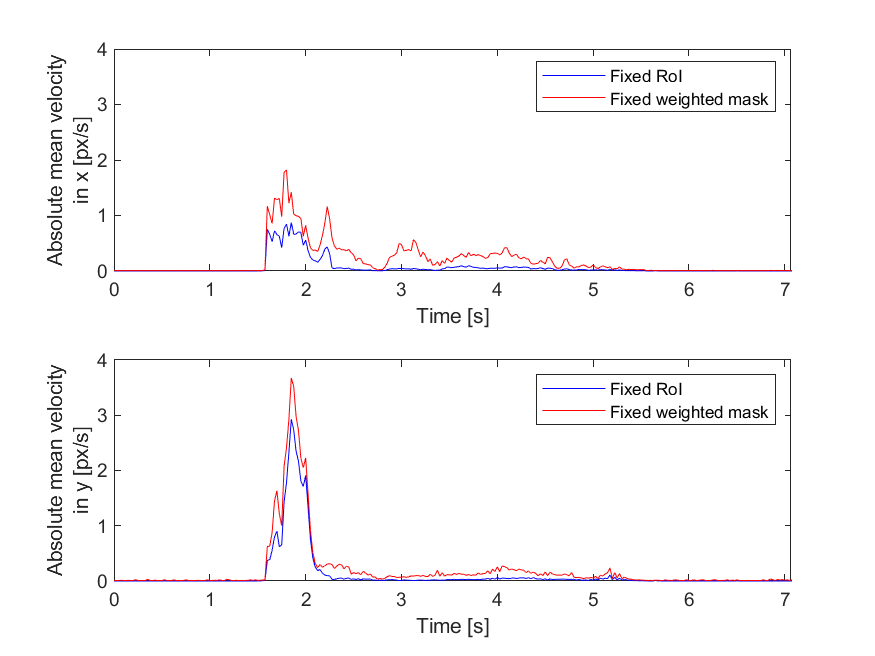
\includegraphics[width=0.95\textwidth]{resources/images/OF_comparison_set_rev}
    \caption{Comparison of the absolute mean velocities' evolution in the whole image for the sequence in ~\Cref{fig:set1_case6}.}\label{fig:OF_comparison_set_rev}
\end{figure}

\begin{figure}[H]
    \centering
    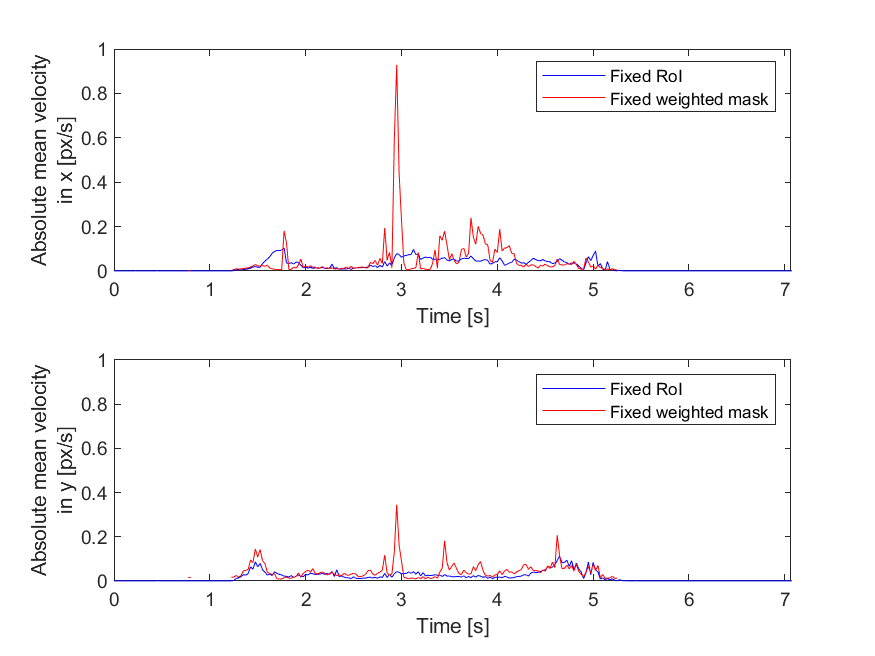
\includegraphics[width=0.95\textwidth]{resources/images/OF_comparison_hb1}
    \caption{Comparison of the absolute mean velocities' evolution in the whole image for the sequence in ~\Cref{fig:set1_case3}.}\label{fig:OF_comparison_hb1}
\end{figure}

Finally, if a highly textured background is present, we saw that the angle of the velocities in the object are not properly estimated, being interpolated from the background. This behavior can also been observed in the velocity signals, depicted in ~\Cref{fig:OF_comparison_hb1_tt}, where the initial peak, corresponding to the slip, is more present in the horizontal axis than the vertical one, while the slip produces vertical motion.

\begin{figure}[H]
    \centering
    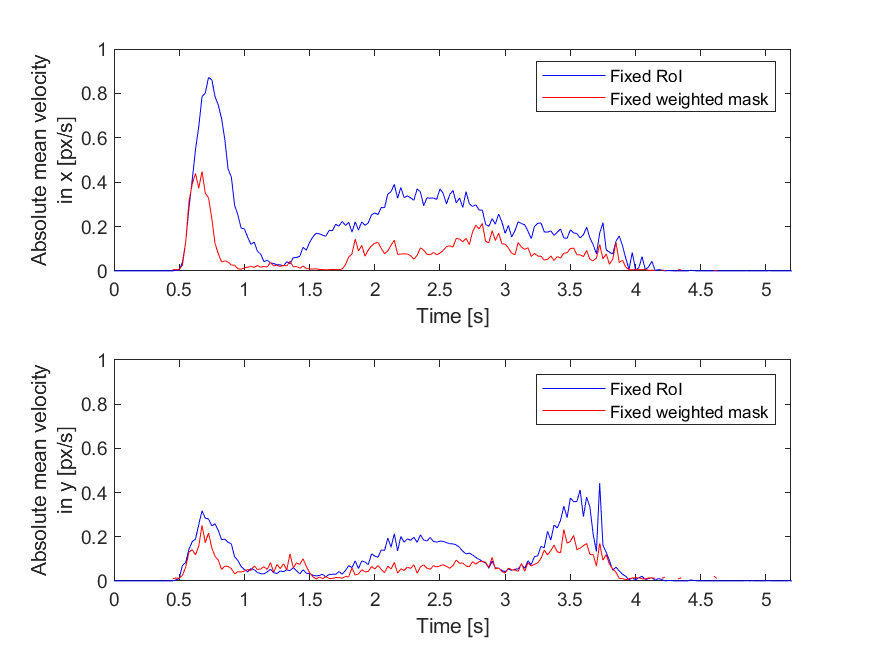
\includegraphics[width=0.95\textwidth]{resources/images/OF_comparison_hb1_tt}
    \caption{Comparison of the absolute mean velocities' evolution in the whole image for the sequence in ~\Cref{fig:set1_case7}.}\label{fig:OF_comparison_hb1_tt}
\end{figure}

\section{Conclusion}

In this chapter two slip detection methods have been analyzed in detail. First, the event rate and ratio signals have been discussed, using different ways of separating the object from the background. The results have shown how the weighted mask and variable mask approaches are more informative and robust to detect rotational slip, compared to the fixed RoI method, which fails in highly textured backgrounds and  sequences where the object's shape changes significantly from the camera's view. Both of them present similar results, but the weighted mask approach is much simpler and does not depend on the prerecorded empty-handed pick-and-place sequence, which may differ from the subsequent experiments, making it quite brittle.\\

Moreover, the optical flow results have been transformed into two 1D signals, the horizontal and vertical absolute mean velocities. These velocities have been computed for the fixed RoI and weighted mask approaches and the results show that the rotational slip coincides, ideally, with high-speed vertical motion in the object. Therefore, it would be enough to threshold the vertical absolute mean velocity signal, in order to detect slip. However, in highly textured backgrounds, the orientation of the motion is not properly estimated, producing the peaks also in the horizontal absolute mean velocity signal. In terms of the methods used to separate the object's motion from the background, the fixed RoI works robustly in all scenarios, while the weighted mask approach fails in one of the experiments, producing false positives.\\

There is no doubt that both presented methods, event rate and optical flow, are informative about rotational slip. However, the designed 1D signals, which were intended to be thresholded and detect slip if the value was above this threshold, are not robust enough to work in different scenarios. In the case of the ratio signal, it is easier to threshold as it is bounded between 0 and 1. On the contrary, the vertical absolute mean velocity signal is not bounded, thus it is more complicated set a limit.\\

All in all, these handcrafted 1D signals are a first step to understand slip detection, but are not enough to generalize in different scenarios and detect slip robustly.






